% Copyright (C) 2013, Tim Felgentreff
% All rights reserved.

% Command to generate a different version of the text for the JOT
% paper and the tech report.  The first argument is the text for the
% JOT paper, the second is for the tec report.
\newcommand\articleORtr[2]{#2}

\providecommand{\printmode}{true}
%%%
\documentclass[tocflat]{scrbook}

\makeatletter


% this is for tim.

\let\subparagraph\paragraph
\let\paragraph\subsubsection
\let\subsubsection\subsection
\let\subsection\section
\let\section\chapter

\iffalse
\let\thesubparagraph\theparagraph
\let\theparagraph\thesubsubsection
\let\thesubsubsection\thesubsection
\let\thesubsection\thesection
\let\thesection\thechapter

\let\addsubparagraphtocentry\addparagraphtocentry
\let\addparagraphtocentry\addsubsubsectiontocentry
\let\addsubsubsectiontocentry\addsubsectiontocentry
\let\addsubsectiontocentry\addsectiontocentry
\let\addsectiontocentry\addchaptertocentry

\let\c@subparagraph\c@paragraph
\let\c@paragraph\c@subsubsection
\let\c@subsubsection\c@subsection
\let\c@subsection\c@section
\let\c@section\c@chapter
\let\p@subparagraph\p@paragraph
\let\p@paragraph\p@subsubsection
\let\p@subsubsection\p@subsection
\let\p@subsection\p@section
\let\p@section\p@chapter
\let\cl@subparagraph\cl@paragraph
\let\cl@paragraph\cl@subsubsection
\let\cl@subsubsection\cl@subsection
\let\cl@subsection\cl@section
\let\cl@section\cl@chapter
\fi

\RequirePackage{expl3}
\RequirePackage{etoolbox}


\RequirePackage{ifthen}
\RequirePackage{ifpdf}
\RequirePackage{ifluatex}
\RequirePackage{ifxetex}


\ifthenelse{\boolean{xetex}}{% xetex
}{ % luatex and pdftex
  \ifthenelse{\boolean{luatex}}{}{
    \RequirePackage[utf8]{inputenc}
  }
  \RequirePackage{cmap}
  \input glyphtounicode
  \pdfgentounicode=1
}

\ifthenelse{\boolean{xetex}}{
  \RequirePackage{polyglossia}

  \ifthenelse{\boolean{@swa@german}}{
    \setotherlanguage{english}
    \setmainlanguage[babelshorthands,latesthyphen=true]{german}
  }{
    \setmainlanguage{english}
    \setotherlanguage[babelshorthands,latesthyphen=true]{german}
  }
  
  \gappto\captionsenglish{%
    \def\figureautorefname{figure}
    \def\tableautorefname{table}
    \def\lstlistingautorefname{listing}
    \def\lstnumberautorefname{line}
    \let\subsectionautorefname\sectionautorefname
    \let\subsubsectionautorefname\sectionautorefname
    }

  \gappto\captionsgerman{%
    \let\subsectionautorefname\sectionautorefname
    \let\subsubsectionautorefname\sectionautorefname
    }
}{
%fool AUCTeX
\iffalse
  \RequirePackage[english]{babel}
\fi

  \RequirePackage%
[ngerman,english]%
%
{babel}
  %//fooling done.

  \addto\captionsenglish{%
    \def\figureautorefname{figure}
    \def\tableautorefname{table}
    \def\lstlistingautorefname{listing}
    \def\lstnumberautorefname{line}
    \let\subsectionautorefname\sectionautorefname
    \let\subsubsectionautorefname\sectionautorefname
    }

  \addto\captionsngerman{%
    \let\subsectionautorefname\sectionautorefname
    \let\subsubsectionautorefname\sectionautorefname
    }

}

\KOMAoptions{
    pagesize,
    DIV=calc,
    appendixprefix=true,
%    footinclude=true
}

\RequirePackage{ifpdf}
\RequirePackage{url}


% macros for comments
\RequirePackage[table,svgnames]{xcolor}
\RequirePackage{color}



\RequirePackage{pdfpages}

%%%
% tocstyle is still alpha
\RequirePackage{tocstyle}
\usetocstyle{KOMAlike}



\ifthenelse{\boolean{xetex}}{}{\pdfcompresslevel=6}

\ifthenelse{\equal{\printmode}{true}}{
  \RequirePackage[bookmarks=false]{hyperref}%
  \hypersetup{
    colorlinks=false, 
    breaklinks=true,
    unicode,%
    final
  }
}{
  \RequirePackage{hyperref}%
  \hypersetup{
    % plainpages=false, %% false, if : destination same identifier already exists
    % pagebackref=true,%
    colorlinks=true,   %% true for printout
    linkcolor=MidnightBlue,%
    citecolor=MidnightBlue,%
    urlcolor=MidnightBlue,%
    breaklinks=true,
    unicode,%
    pdfstartpage=3,
    % pdfpagescrop={92 112 523 778}, % LNCS paper size
    final
  }
}


% Disable single lines at the start of a paragraph (Schusterjungen)
\clubpenalty = 10000
% Disable single lines at the end of a paragraph (Hurenkinder)
\widowpenalty = 10000 
\displaywidowpenalty = 10000 % formulas
\setlength{\textfloatsep}{\baselineskip}
\setlength{\floatsep}{\baselineskip}

\setfootnoterule{4cc}

\frenchspacing
\raggedbottom

% Better float parameters: (from the TeX FAQ)
\renewcommand{\topfraction}{.85}
\renewcommand{\bottomfraction}{.7}
\renewcommand{\textfraction}{.15}
\renewcommand{\floatpagefraction}{.66}
\renewcommand{\dbltopfraction}{.66}
\renewcommand{\dblfloatpagefraction}{.66}
\setcounter{topnumber}{9}
\setcounter{bottomnumber}{9}
\setcounter{totalnumber}{20}
\setcounter{dbltopnumber}{9}


%\RequirePackage[hang,small,bf]{caption}
\setcapindent{1em}
\addtokomafont{caption}{\small}
\addtokomafont{captionlabel}{\bfseries}


% \RequirePackage{enumitem}
% \setlist{noitemsep,topsep=0pt,partopsep=0pt}
% \setdescription{noitemsep,font=\normalfont\scshape,leftmargin=\parindent}
% \setlist[1]{leftmargin=0pt}
% \setitemize[1]{label=\footnotesize\textbullet}

%%
%% An Asterism (three * arranged triangularly)
%% works well as separator.
%%
\newcommand{\asterism}{\smash{% 
    \raisebox{-.5ex}{% 
      \setlength{\tabcolsep}{.75pt}% 
      \begin{tabular}{@{}cc@{}}% 
        \multicolumn2c*\\[-1.75ex]*&*% 
      \end{tabular}}}}
\providecommand\vskipnextgrid{\vskip\baselineskip}
\newcommand{\ParSep}{{\vskipnextgrid\noindent\hbox to \textwidth{\hss\large\asterism\hss}\par\vskipnextgrid}}

\RequirePackage{pifont}
% Table stuff
\RequirePackage{longtable}
\RequirePackage{ctable}
% ctable is dumb sometimes
\renewcommand{\tmark}[1][a]{%
  \rlap{\hbox{\@textsuperscript{\rmfamily\itshape #1}}}}


\providecommand*\tablefontcommand{}
\providecommand*\tableinsidecommand[1][2]{%
  \def\y{\ding{52}\relax\xspace}\relax%
  \def\n{\ding{56}\relax\xspace}\relax%
  \smaller\rowcolors*{#1}{light}{white}\tablefontcommand%
}
\setupctable{pos=htbp,doinside=\tableinsidecommand,table,notespar}

\KOMAoptions{
    open=any,
}

% Graphics
\RequirePackage{graphicx}

% Figures/Floats, often used with graphic
%\RequirePackage{subfig}
\RequirePackage{wrapfig}

\RequirePackage{tikz}
\RequirePackage{pgfplots}
\pgfplotsset{compat=1.5.1} 

\RequirePackage[final]{listings}
\RequirePackage{relsize}

\providecaptionname{english}{\lstlistlistingname}{List of Listings}
\providecaptionname{german}{\lstlistlistingname}{Listingverzeichnis}
\providecaptionname{ngerman}{\lstlistlistingname}{Listingverzeichnis}
% \renewcaptionname{english}{\lstlistlistingname}{List of Listings}
% \renewcaptionname{german}{\lstlistlistingname}{Listingverzeichnis}
% \renewcaptionname{ngerman}{\lstlistlistingname}{Listingverzeichnis}

\providecommand{\listingnumberfont}{{}}
\lstset{numberstyle=\listingnumberfont}

\newcommand{\swaListingInlineMode}{
  \lstset{%
    columns=fullflexible,
    basicstyle=\ttfamily
  }}

\newcommand{\swaListingMode}{
  \lstset{%
    columns=[c]fixed,
    basicstyle=\smaller\ttfamily,
  }}

\swaListingInlineMode

% \lstnewenvironment{code}[3][]%
% {
% \swaListingMode
% \lstset{
% label=#1,
% caption={#2},
% #3
% }}{
% \swaListingInlineMode
% }


% packages
\RequirePackage{textcomp}
\RequirePackage{textcase}
\RequirePackage{fontaxes}
\RequirePackage{relsize}

\RequirePackage[final,babel=true]{microtype}[2011/08/18]

%
% engine-dependent, eg, encoding, loading.
%
\ifthenelse{\boolean{luatex} \or \boolean{xetex}}{%
  \RequirePackage{fontspec}
  \ifthenelse{\boolean{xetex}}{
    \newfontfeature{Microtype}{protrusion=default;expansion=default;}
  }{
    \newfontfeature{Microtype}{}
  }
}{
  \RequirePackage[T1]{fontenc}
}

%
% Set a Vera mono/DejaVu descendant as monofont.
%
\ifthenelse{\boolean{luatex} \or \boolean{xetex}}{%
  \setmonofont%
     [Scale=MatchLowercase,Microtype,Ligatures=TeX]%
     {DejaVu  Sans Mono}%
   \defaultfontfeatures{Numbers=OldStyle,Microtype,Ligatures=TeX,RawFeature={+calt,+clig,+tlig}}
}{
  \RequirePackage[scaled=.9]{beramono}
}


\ifthenelse{\boolean{xetex}}{
   \AtBeginDocument{%
     \def\mainfontlist{Palatino Linotype,TeX Gyre Pagella,Palatino}

     \edef\RestoreErrorConditions{%
       \suppressfontnotfounderror=\the\suppressfontnotfounderror\relax
       \interactionmode=\the\interactionmode\relax
     }
     \suppressfontnotfounderror=1 %
     \batchmode
     \newif\ifpalatinofound
     \@for\next:=\mainfontlist\do{%
       \ifpalatinofound\else
         \font\x="\next" at 10pt
         \ifx\x\nullfont%
         \else
           \xdef\fonttouse{\next}
           \PackageInfo{swa-font-palatino}{Using `\next' as Palatino.}
           \global\palatinofoundtrue
          \fi
       \fi
      }
      \RestoreErrorConditions
      \setmainfont{\fonttouse}
      \edef\palaLino{Palatino Linotype}
      \ifx\fonttouse\palaLino%
      \ExplSyntaxOn
      \RenewDocumentCommand \liningnums {m}
      {%
        {\addfontfeature{RawFeature={-onum}}#1}
      }%
      \ExplSyntaxOff
      \else\fi
    }
}{}

\ifthenelse{\boolean{luatex}}{%
  \setmainfont{TeX Gyre Pagella}
}{}

\ifthenelse{\boolean{xetex} \or \boolean{luatex}}{}{%
  \RequirePackage[osf,sc]{mathpazo} % Palatino with real small caps and old style figures
}


\linespread{1.05} % a bit more for Palatino
% math font: euler
\RequirePackage[euler-digits,T1]{eulervm}


%
% microtypesetup
%
\ifthenelse{\boolean{xetex}}{%
  \microtypesetup{protrusion}
  \let\textls\undefined
  \DeclareRobustCommand{\textls}[2][80]{%
    {{\addfontfeature{LetterSpace=\the\numexpr#1/10\relax}#2}}}
}{}

\ifthenelse{\boolean{luatex}}{%
  \microtypesetup{protrusion,tracking}
}{}

\ifthenelse{\boolean{xetex} \or \boolean{luatex}}{}{%
  \microtypesetup{stretch=9,shrink=15,step=3,tracking=smallcaps,letterspace=75}
}

%
% useful commands
%
\DeclareRobustCommand{\spacedallcaps}[1]{%
  \textls[80]{\MakeTextUppercase{#1}}}%
\DeclareRobustCommand{\spacedlowsmallcaps}[1]{%
  {\MakeTextLowercase{\scshape #1}}}%s
\DeclareRobustCommand\Largespacedlowsmallcaps[1]{%
  \spacedlowsmallcaps{\Large    #1}}


%
% design
%
\setkomafont{subtitle}{\usekomafont{title}\LARGE}
%\setkomafont{disposition}{\rmfamily\mdseries\scshape}
\addtokomafont{disposition}{\rmfamily}
\setkomafont{title}{\rmfamily\mdseries}

\@ifundefined{abstract}{
\newenvironment{abstract}{}{}
}{}
\@ifundefined{zusammenfassung}{
\newenvironment{zusammenfassung}{}{}
}

%% XXX: review here

\ifthenelse{\boolean{xetex}}{
  \renewenvironment{abstract}{%
    \begingroup
    \let\raggedsection\centering
    \begin{english}
    \chapter*{\abstractname}
  }{%
    \end{english}
    \endgroup
  }
  \renewenvironment{zusammenfassung}{%
    \begingroup
    \let\raggedsection\centering
    \begin{german}
    \chapter*{\abstractname}
  }{%
    \end{german}
    \endgroup
  }
}{%%% non-xetex uses babel.
  \renewenvironment{abstract}{%
    \begingroup
    \let\raggedsection\centering
    \selectlanguage{english}
    \chapter*{\abstractname}
  }{%
    \endgroup
  }
  \renewenvironment{zusammenfassung}{%
    \begingroup
    \let\raggedsection\centering
    \selectlanguage{ngerman}
    \chapter*{\abstractname}
  }{%
    \endgroup
  }
}

% koma-hacks
\RequirePackage{scrhack}

% undo babel thing in tocbasic
\unsettoc{toc}{nobabel}
\unsettoc{lof}{nobabel}
\unsettoc{lot}{nobabel}

\setuptoc{toc}{noprotrusion}
\setuptoc{lof}{noprotrusion}
\setuptoc{lot}{noprotrusion}
\setuptoc{lol}{noprotrusion}
\setuptoc{loa}{noprotrusion}

\tocbasicautomode

\newcommand\hairspace{\ifmmode\mskip1mu\else\kern0.08em\fi}
\RequirePackage{xspace}



%\recalctypearea
\raggedbottom

%redo document stuff:

\ifundefinedorrelax{hypersetup}{}{%
  \AtEndPreamble{
    \begingroup
      \let\and\space
      \xdef\clean@author{\@author}
    \endgroup
    \hypersetup{
      pdftitle={\@title{}: \@subtitle},
      pdfauthor={\clean@author},
      pdfsubject={\@subject}
    }
  }
}

\makeatother

%%% Local Variables:
%%% mode: latex
%%% End:


\usepackage{subcaption}

\usepackage{array} % tables
\usepackage{afterpage} % figures
\usepackage{float} % figures
\usepackage{paralist} % figures
\usepackage[shortcuts]{extdash} % figures
\usepackage{todonotes}
\usepackage{lmodern}
\lstset{%
  language=ruby,%
  basicstyle=\scriptsize,%\ttfamily,
  frame=single,%
  emph={always, once, constructor},%
  emphstyle=\bfseries,%
  % breaklines=true,
  breakatwhitespace=false,%
  literate={<<}{\tiny{$\ll$}~}{1}%
  {.?}{\bfseries\emph{.?}}{1}%
  {visible?}{visible?}{1},%
  showstringspaces=false,%
  columns=flexible}
\lstnewenvironment{code}[1][]%
{\vskip0em\noindent
  \minipage{\linewidth}
  \vspace{0.5\baselineskip}
  \lstset{%
    language=ruby,%
    basicstyle=\scriptsize,%\ttfamily,
    frame=single,%
    emph={always, once, constructor},%
    emphstyle=\bfseries,%
    % breaklines=true,
    breakatwhitespace=false,%
    literate={<<}{\tiny{$\ll$}~}{1}%
             {.?}{\bfseries\emph{.?}}{1}%
             {:x}{:x}{1}%
             {:y}{:y}{1}%
             {:high}{:high}{1}%
             {:low}{:low}{1}%
             {visible?}{visible?}{1},%
    showstringspaces=false,%
    columns=flexible,#1}}
{\endminipage\vskip0em}

\restylefloat{figure}

\usepackage{glossaries}
\newcommand{\ac}[1]{\gls{#1}}
\newcommand{\acp}[1]{\glspl{#1}}

% Acronyms
\newacronym{api}{\textsc{api}}{application programming interface}
\newacronym{cip}{\textsc{cip}}{constraint imperative programming}
\newacronym{ocp}{\textsc{ocp}}{object constraint programming}
\newacronym{oo}{\textsc{oo}}{object-oriented}
\newacronym{dsl}{\textsc{dsl}}{domain specific language}
\newacronym{frp}{\textsc{frp}}{functional reactive programming}
\newacronym{vm}{\textsc{vm}}{virtual machine}
\newacronym{jit}{\textsc{jit}}{just-in-time}

\newcommand{\eg}{e.\hairspace{}g.,\xspace}
\newcommand{\Eg}{E.\hairspace{}g.,\xspace}
\newcommand{\Ie}{I.\hairspace{}e.,\xspace}
\newcommand{\ie}{i.\hairspace{}e.,\xspace}
\newcommand{\cf}[1]{cf.\,{#1}\xspace}
% \newcommand{\todo}[1]{\framebox{\textsc{todo} #1}}

\newcommand{\zthree}{Z3\xspace}
\newcommand{\langname}{\textsc{Babelsberg}\xspace}
\newcommand{\toolname}{\textsc{Babelsberg/R}\xspace}

\newcommand{\load}{\textsc{load}\xspace}
\newcommand{\store}{\textsc{store}\xspace}

\def\sectionautorefname{Section}
\def\subsectionautorefname{Section}
\def\subsubsectionautorefname{Section}
\def\tableautorefname{Table}
\def\figureautorefname{Figure}

\title{Babelsberg: Specifying and Solving Constraints on Object Behavior}


\begin{document}
\makeglossaries

\begin{abstract}
  Constraints allow developers to specify desired properties of
  systems in a number of domains, and have those properties be
  maintained automatically.  This results in compact, declarative
  code, avoiding scattered code to check and imperatively re-satisfy
  invariants.  Despite these advantages, constraint programming is not
  yet widespread, with imperative programming still the norm.

  There is a long history of research on integrating
  constraint programming with the imperative
  paradigm. However, this integration typically does not unify the
  constructs for encapsulation and abstraction from both
  paradigms. This impedes re-use of modules, as client code written in
  one paradigm can only use modules written to support that
  paradigm. Modules require redundant definitions if they are to be
  used in both paradigms.

  We present a language -- \langname~-- that unifies the constructs
  for encapsulation and abstraction
  by using only object-oriented method definitions
  for both declarative and imperative code. Our prototype --
  \toolname~-- is an extension to Ruby, and continues to support
  Ruby's object-oriented semantics.  It allows
  programmers to add constraints to existing Ruby programs in
  incremental steps by placing them on the results of normal
  object-oriented message sends.  It is implemented by modifying
  a state-of-the-art Ruby virtual machine.  The performance of standard
  object-oriented code without constraints is only modestly impacted,
  with typically less than 10\% overhead compared with the unmodified
  virtual machine. Furthermore, our architecture for adding multiple
  constraint solvers allows \langname to deal with constraints in a
  variety of domains.

  We argue that our approach provides a useful step toward making
  constraint solving a generic tool for object-oriented programmers.
  We also provide example applications, written in our Ruby-based
  implementation, which use constraints in a variety of application
  domains, including interactive graphics, circuit simulations, data
  streaming with both hard and soft constraints on performance, and
  configuration file management.

  % We present an approach and extension to an object-oriented language
  % to solve constraints on the results of message sends. These
  % constraints are predicates that are continuously maintained by the
  % system.

  % Constraints are written as anonymous functions that contain
  % constraint expressions. To maintain a constraint, our approach
  % chooses a constraint solver based on the return types of the
  % messages sent in the dynamic extent of the expression execution.
  % Solvers can be flexibly bound to types such as reals or strings, but
  % also complex objects such as files or methods. Furthermore,
  % constraint solvers are implemented in application code, so
  % programmers can add domain specific solvers for their use cases.

  % Our system solves constraints by modifying objects that determine
  % the results of messages sent during the constraint expression
  % execution. Whenever imperative code changes these objects, the
  % appropriate solvers are triggered to maintain the constraints.

  % Our approach is superior to existing approaches because it relies on
  % object-oriented message sends instead of paths between objects or
  % special constraint method definitions. This property ensures both
  % encapsulation and supports the uniform access principle. This, in
  % turn, allows programmers to change the implementation of objects
  % without breaking constraint code, as well as applying groups of
  % constraints to different objects that implement the same
  % interface. Since programmers can extend the available solvers, they
  % can choose the solver that gives the best results or provides the
  % best performance to their specific application.

  % We argue that using our approach, constraint solving becomes a
  % generic tool that is not limited to specific domains. Using a
  % Ruby-based implementation, we show example applications that apply
  % constraints to interesting new domains such as performance
  % assurances and configuration file handling.

\end{abstract}

%%% Local Variables: 
%%% mode: latex
%%% TeX-master: "babelsberg_jot"
%%% End: 


\tableofcontents
% \listoffigures
% \listoftables
% \lstlistoflistings

\section{Introduction}
\label{sec:introduction}

  % % Context
  % Imperative object-oriented programming languages are ill-suited to
  % describe constraints between objects. They require programmers to
  % maintain the constraints explicitely through assignments and control
  % flow scattered throughout the code, rather than declare them in one
  % place. For some specific problem domains---such as graphical
  % layouting or musical harmonization ---specialized constraint
  % libraries provide solutions to this issue. For general purpose
  % applications, constraint-oriented extensions to imperative languages
  % have been explored.

  % % Problem
  % However, current approaches result in unsatisfactory trade-offs
  % between constraint-oriented and object-oriented programming. They
  % either violate object encapsulation by defining constraints only on
  % state, do not integrate constraint solving and the object-oriented
  % behavior definition into one language, and/or are limited to
  % specific domains. Consequently, current approaches increase coupling
  % in the system, duplicate definitions of relations across behavior as
  % well as constraint-expressions, and/or are not directly reuseable
  % for new domains.

  % % Solution
  % We present an extension to an object-oriented language that allows
  % developers to apply constraints to complex objects and the results
  % of message sends to them. Our approach preserves encapsulation and
  % re-uses the existing object-oriented method definitions for the
  % constraint declarations. Our system can deal with constraints on
  % complex objects (by automatically destructuring them) and provides
  % extension points so users can define specialized constraint solvers
  % for specific domains.

Constraints and constraint programming occur in a variety of
application domains within computer science and related fields,
including graphics, CAD/CAM, planning and operations research,
artificial intelligence, user interface toolkits, and programming
languages. A \emph{constraint} in these domains is a relation that
should hold, for example: that there be a minimum of 10 pixels
horizontal space between two buttons on a screen, that a resistor in
an electrical circuit simulation obey Ohm's Law, that a maximum of 10
parts per hour can be produced by a machine in a factory, that all of
the digits in a row or column or subregion of a Sudoku puzzle must be
different, or that the height of a bar in a bar chart correspond to a
value produced by a simulation. Constraints are declarative: they
specify \emph{what} should be the case rather than \emph{how} to
achieve it.  They thus provide flexibility in the way they can be
employed, because the \emph{how} can be exchanged.

A number of features are desirable in constraint programming to solve
a useful set of problems.  Given a collection of constraints over
variables in different type domains --- such as floats, integers,
booleans, or complex objects --- it is unrealistic to expect a single
solver to work efficiently for all of these constraints, as finding a
solution to a constraint satisfaction problem is NP-complete in the
general case~\cite{cook1971complexity}. More efficient solvers impose
restrictions on the kinds of constraints they can solve, for example,
by supporting only floats and not integers or requiring numeric
equalities to be linear. So, in general, a variety of solvers are
needed, depending on the type domain and particular characteristics of
the constraints.  It is also useful to have these solvers interoperate
to find a solution to a particular problem. Furthermore, in some
application domains, it is useful to support soft as well as hard
constraints, that is, constraints that should be satisfied if possible
and constraints that must be satisfied. Finally, in the presence of
frequent changes incremental solvers are required that can efficiently
re-solve a set of constraints.  Interactive graphical systems are an
example of all of these: they include constraints on complex objects
such as points and areas as well as floats and integers, soft
constraints to express preferences regarding the layout, and require
incremental solvers to efficiently re-solve constraints repeatedly
as a part of the figure is moved.

There are two main options how to use constraints in imperative
programs. The most common way is via a constraint satisfaction
library.  This means that no changes are required to the underlying
programming language, but has the disadvantage that, besides writing
the constraints, the solver needs to be explicitly invoked at
appropriate times during the execution. If it is not, the programmer
may inadvertently ignore or bypass the constraints.  An alternate
technique is to support constraints directly in the underlying
programming language.  This addresses the problem of inadvertently
bypassing the constraint system, because the programming language
ensures that the solver is invoked whenever neccessary. This approach
also typically provides a more convenient syntax for writing
constraints, either using a separate \ac{dsl} embedded in the host
language (with the drawback of having to learn essentially two
programming languages), or (as in the work reported here) by allowing
constraints to be written in the host language itself, of course at
the cost of having to support a new or extended programming
language.

Prior approaches of the latter kind typically provide a unified
runtime, a semantics for the interactions between declarative and
imperative code, and a linguistic symbiosis. As an extension of these,
this work additionally unifies the programming constructs for
encapsulation and abstraction by using only object-oriented methods,
classes, and inheritance for defining behavior and structure in both
the imperative and declarative paradigm.

We present our design for integrating constraints with a standard
object-oriented language that preserves a familiar imperative
programming model, called \langname, and describe an implementation of
that design as an extension to Ruby~\cite{flanagan2008ruby}, called
\toolname. Key contributions for \langname with respect to language
design are as follows.

\begin{itemize}
\item The semantic model for \langname is a direct extension of a
  standard object-oriented model (with dynamic typing, object
  encapsulation, and standard classes, instances, methods, and message
  sends).  It supports placing constraints on the results of message
  sends rather than just on object attributes --- thus, we argue,
  being more compatible with object-oriented encapsulation and
  abstraction.
\item The syntax of \langname is a strict superset of that of the base
  language, with only one minor extension, making it easy for the
  programmer to write and read constraints and object-oriented code.
\item \langname includes constructs that allow specifying soft as well
  as hard constraints, and that support incremental solving.
\end{itemize}

%% this is deleted for now, until it is supported:
%% that supports multiple cooperating constraint solvers,

Additional contributions with respect to implementation techniques are
as follows.

\begin{itemize}
\item We present a technique for implementing object constraint
  languages, which uses a primitive to switch the interpreter between
  imperative evaluation, constraint construction, and constraint
  solving modes.  In imperative evaluation mode, the interpreter
  operates in the standard fashion, except that \load and \store
  operations on variables with constraints obtain the value from the
  constraint solver or send the new value to the solver (which may
  trigger a cascade of other changes to satisfy the constraints).  In
  constraint construction mode, the expression that defines the
  constraint is evaluated, not for its value, but rather to build up a
  network of primitive constraints that represent the constraint being
  added.  The interpreter keeps track of dependencies in the process,
  so that, as needed, the solver can be activated or the code to
  construct the constraint can be re-evaluated.
\item \langname provides an architecture for constraint solvers that
  supports multiple constraint solvers, which makes it straightforward
  to add new solvers, and that does not privilege the solvers provided
  with the basic implementation (they are simply the solvers that are
  in the initial library).
\item We describe a working prototype system, integrated with a state
  of the art Ruby virtual machine and \ac{jit} compiler. In the
  absence of constraints, the performance of a program written in the
  host language (Ruby) is only modestly impacted.
\end{itemize}

\toolname is a general-purpose object constraint language, and we have
implemented a variety of example programs, including a video streaming
example with both hard and soft constraints on performance,
interactive graphical layout examples (which exercise soft constraints
and incrementality), electrical circuit simulations, and solvers for
puzzles such as Eight Queens and cryptarithmetic.

\section{Background and Related Work}
\label{sec:background-related-work}

%% possible reorganization:
%% describe different kinds of constraints
%% describe solvers
%% divide constraint systems into one way vs multi-way

%% libraries vs. integration with programming language
%% what kind of language
%%   logic programming
%%   object-oriented

Programs frequently have some set of constraints that should hold.
For standard imperative languages, the usual approach to dealing with
such constraints is to leave it entirely up to the programmer to
ensure that they are satisfied --- the constraints are either just in
comments and documentation, or perhaps in the form of
machine-checkable assertions.  For the latter case, programmers
typically write assertions to fail early if these constraints are
unexpectedly not satisfied~\cite{rinard2005exploring}.

Consider a rectangle implemented as a pair of points, as in the
following code.  The rectangle is displayed in an application window
which the user can resize.  Suppose this rectangle encompasses some
information that we want to make sure remains visible. We want to make
sure the area of the rectangle is never less than 100 square pixels
and that its origin is always within display bounds,
\ie non-negative.  (It would be straightforward to include two
additional tests that \lstinline{corner.x<=DISPLAYWIDTH} and
\lstinline{corner.y<=DISPLAYHEIGHT}; these are omitted for simplicity
since the \lstinline{visible?} method already demonstrates conjunctive
constraints.)

\begin{code}
class Rectangle
  attr_accessor :origin, :extent

  def visible?
    origin.x >= 0 and origin.y >= 0
  end

  def area
    extent.x * extent.y
  end
end
\end{code}

%% Was a floating figure - we should treat this uniformly.  Here I
%% made it inline.

Imperatively, we can use, for example, aspects to satisfy these
constraints explicitly whenever the rectangle changes:
\begin{code}
class RectAspect < Aspect
  def ensure_constraints(method, rect, status, *args)
    rect.origin.x = 0 if rect.origin.x < 0
    rect.origin.y = 0 if rect.origin.y < 0
    rect.extent.x = 100.0 / rect.extent.y if rect.area < 100
  end
end

RectAspect.new.wrap(Rectangle, :postAdvice, /(origin|extent)=/)
\end{code}

However, the above code has a number of problems:
\begin{itemize}
\item The original constraints are expressed in a form that makes them
  harder to understand.
\item Advice code is required to capture all modifications that may
  invalidate the constraints --- if the advice is insufficient or not
  executed at the correct times, the constraints may be violated
  through parts of the execution.
\item There are actually multiple possible solutions to the
  constraints, but which one should be selected is not represented
  explicitly, but instead is implicit in the code.  (For example, a
  rectangle with area 200 instead of 100 would also satisfy the
  minimum area constraint.)  Since there isn't a declarative
  specification of what an optimal solution is, it is nontrivial to
  decide whether the solution is optimal. In the presence of competing
  soft constraints, \ie multiobjective optimizations, this becomes
  even harder.
\end{itemize}

\subsection{Constraint Satisfaction Libraries}

Thus, it is usually clearer to express and satisfy the constraints
explicitly.  One approach is to use a library that provides one or
more constraint solvers, and that can be called directly from the
imperative code.  There is a huge range of such solvers.  One way of
classifying solvers is by the type domain of the constraints (for
example, real numbers or finite domains or arbitrary objects); whether
the solver can use the constraints in a general way (\eg for $c=a+b$,
to solve for any of $a$, $b$, or $c$; or as a dataflow constraint, \ie
to only use the constraint to find a value for $c$); and whether the
solver supports soft constraints as well as hard (required) ones.

A few solvers of particular note to the programming language community
are \zthree~\cite{de2008z3}, a state-of-the-art SMT solver from
Microsoft Research designed for theorem proving (\eg for program
verification), and kodkod~\cite{torlak2007kodkod} for constraints over
finite domains.  For use in interactive graphics systems, include
Cassowary~\cite{badros-tochi-2001}, an incremental solver for linear
equality and inequality constraints that supports soft constraints as
well as hard ones; the Aukland Layout Editor~\cite{lutteroth2008end},
which includes support for a GUI builder using constraints, and
earlier work on DeltaBlue~\cite{freeman-benson-phoenix-1989}, which
supports multi-way local propagation constraints and soft constraints.
There is also a range of commercial application of such solvers, such
as the CPLEX optimizer for mathematical
programming~\cite{optimization1993using}.

For example the following code rewrites the previous, purely imperative
solution to use the \zthree constraint solver to solve our
constraints:
\begin{code}
class RectAspect < Aspect
  def ensure_constraints(method, rect, status, *args)
    ctx = Z3::Context.new
    ctx << Z3::Variable.new("extent_x", rect.extent.x)
    ctx << Z3::Variable.new("extent_y", rect.extent.y)
    ctx << Z3::Constraint.new("extent_x * extent_y >= 100")
    # ... same for origin constraint
    ctx.solve
    rect.extent.x = ctx["extent_x"]
    rect.extent.y = ctx["extent_y"]
  end
end
# boilerplate code as for purely imperative approach
\end{code}

Using a solver allows programmers to express constraints about the
system in terms of a solver-specific type domain (\eg reals, booleans,
uninterpreted function symbols) the solver understands. If the problem
is expressible in a type domain for which a solver is available (as
the above code is) the constraints can be clearly written.

\subsection{Domain-specific Languages for Constraints}

For specialized application domains such as user interface layout,
constraints are sometimes available via a separate \ac{dsl} that
describes relations between visible objects that can be automatically
maintained by the runtime.  Examples of such \acp{dsl} are
\textsc{css}~\cite{lie-css-book}, the Mac OS
X~\cite{AppleCocoaAutoLayout} layout specification language (which
uses Cassowary to solve the constraints), and the Python GUI framework
\emph{Enaml}~\cite{Enaml}. These allow programmers to express
relations such as distances between objects or parent/child
alignments. These constraints are automatically re-satisfied by the
runtime when imperative code changes the user interface.

The following is an example of an \emph{Enaml} specification for our
problem:
\begin{code}[language=python]
enameldef Main(Window):
    Container:
        constraints = [
            # the rectangle area is called contents in enamel
            contents_top >= 0, contents_left >= 0,
            (contents_bottom - contents_top) *
              (contents_right - contents_left) >= 100
        ]
\end{code}

This approach allows programmers to specify constraints and avoid
boilerplate code to trigger constraint solving, and has found
widespread adoption and renewed interest recently in particular
through the Mac OS X layout system.

\subsection{Dataflow Constraints and FRP}

Some languages have built-in support for data flow, which allows
programmers to express unidirectional constraints between objects and
their parts. Examples of such systems are
Scratch~\cite{resnick2009scratch},
LivelyKernel/Webwerkstatt~\cite{lincke2012lively}, or
KScript~\cite{ohshima2012report}.

The following uses LivelyKernel connections to observe changes to
\texttt{origin} and \texttt{extent} in a Rectangle \texttt{rect}.  On
each change, the transformation function is executed with the current
and the previous value and returns the new value for the
field. Programmers can thus directly express relations between
objects.
\begin{code}[language=java]
connect(rect, "origin", rect, "origin",
        function(origin, prevOrigin) {
            if (this.isVisible()) return prevOrigin;
            else return origin;
        })
connect(rect, "extent", rect, "extent",
        function(extent, prevExtent) {
            if (this.area() < 100) return prevExtent;
            else return extent;
        })
\end{code}

Although these systems are not constraint solvers, programmers can use
constraint solvers (in the hook function passed to
\lstinline{connect}) to calculate new values and some systems, like
KScript, already integrate a constraint solver to use in the
connection. These approaches answer the question when to trigger
constraint solving.

\subsection{Integrating Constraints with a Programming Language}

Another approach to supporting constraints --- and the one adopted in
the work reported here --- is to integrate this support with the
programming language itself.  Again, there is a substantial body of
prior work in this area.  

One of the most widely known of these approaches evolved from logic
programming, for example the Constraint Logic Programming
scheme~\cite{jaffar-popl-1987} and instances of this scheme such as
CLP($\cal R$)~\cite{jaffar-toplas-1992} (which provides constraints
over real numbers). The CLP languages are in the logic programming
family, and in their standard form have no notion of state or state
change.  Other languages of this kind include Concurrent Constraint
Programming~\cite{saraswat-book}.

Such languages have significant advantages, such as a clean semantics,
but at the same time sacrifice familiar capabilities and programming
style.  Our goal here is to support a more standard object-oriented,
imperative programming style and syntactic integration of constraint
and imperative programming.  With these goals, \langname follows the
work by Freeman-Benson, Lopaz, and Borning on
\ac{cip}~\cite{freeman-benson-ecoop-1992,lopez-ecoop-1994,lopez-oopsla-1994,lopez-asi-1994}
and the Kaleidoscope language. Systems related to Kaleidoscope include
Siri~\cite{horn-oopsla-1992}, Turtle~\cite{grabmuller2004turtle}, and
\textsc{Soul}~\cite{d2004seamless}. BackTalk~\cite{roy1997reifying} is
another system that aims to integrate a rich set of constraint solvers
with imperative languages, but without syntactic integration.

There is also a body of work that uses constraints in other ways in
standard programming languages.  For example, in Plan B, Samimi, Aung, and
Millstein \cite{samimi-ecoop-2010} use specifications as ``reliable
alternatives'' to implementations, so that if an assertion fails, the
system can use the specification as input to a constraint solver and
continue execution.  Similarly, Demsky and Rinard~\cite{demsky2006goal}
use constraint solvers to correct a faulty program state automatically
and continue running.  (Thus, by replacing assertions with
constraints, undesirable program states can be corrected by the
runtime.)

\subsubsection*{Constraint-Imperative Programming in Kaleidoscope}
Because the current work shares many of its motivations with
Kaleidoscope, it also shares important design aspects that were
developed over the iterations of the Kaleidoscope language.

Kaleidoscope supported standard classes and instances, and in
addition, integrated constraints with the language itself.  To support
this, it included built-in constraints over primitive objects (such as
floats) and constraints over user-defined objects, which were provided
by \emph{constraint constructors}.  For example, the \lstinline{+}
constraint for Points could be defined using a constraint constructor
\lstinline{a+b=c} that then expanded this into constraints on the
\lstinline{x} and \lstinline{y} instance variables of the three points
\lstinline{a}, \lstinline{b}, and \lstinline{c}.  Separately, the
language also provided methods.  Both constraint constructors and
standard methods were selected using multi-method semantics.  This
accommodated, for example, the case of a constraint constructor call
\lstinline{a+b=c} in which \lstinline{b} and \lstinline{c} were known
and \lstinline{a} was unknown.

In contrast to Kaleidoscope, \langname provides a simpler semantic
model directly extending a standard object-oriented model with
ordinary methods using standard object-oriented message dispatch,
rather than special constraint constructors and multi-methods.  The
implementation includes an integration with a state of the art virtual
machine and \ac{jit}, so that in the absence of constraints, the
performance of a program written in the host language is unaffected.

This work's treatment of mutable state and time in \langname is very
similar to the later incarnations of Kaleidoscope. The first version
of Kaleidoscope, Kaleidoscope'90~\cite{freeman-benson-iccl-1992}, used
a \emph{refinement} model, in which variables held a stream of values,
related to each other by constraints.  Variables typically had a
low-priority \emph{stay} constraint so that they retained their value
over time, \eg \mbox{$x_t = x_{t-1}?$}.  (The question mark is a
read-only annotation: the constraint solver wasn't allowed to change
the past to satisfy constraints on the present.)  There were
facilities to access both the current and previous states of a
variable.  Object identity was only an implementation issue in
Kaleidoscope'90, and not semantically significant, because a variable
would never change its identity (it was a stream uniquely identified
by its name), but only assume different values over time. Later
versions of the language (\eg Kaleidoscope'93)
\cite{lopez-ecoop-1994,lopez-oopsla-1994} switched to a
\emph{perturbation} model, in which destructive assignment can change
the state of objects (perhaps making previously satisfied constraints
unsatisfied), and the system perturbs or adjusts values to reach a new
state that best satisfies the constraints. Instead of streams of
values, a variable in Kaleidoscope'93 referred to a single object, as
in a more conventional languages.  Kaleidoscope'93 also made object
identity a part of the language semantics, including support for
identity constraints as well as equality constraints.

%% add note about multiple cooperating solvers if implemented

%% Our rectangle example can be expressed using Kaleidoscope as follows:
%% \begin{code}
%% class Rectangle
%%   constructor area = (n: Integer)
%%     always: extent.x * extent.y = n
%%   end

%%   constructor visible?
%%     always: origin.x >= 0
%%     always: origin.y >= 0
%%   end
%% end

%% rect = Rectangle.new
%% always: rect.area = 100
%% always: rect.visible?
%% \end{code}

%% The above code states constraints clearly, and \emph{constraint
%%   constructors} modularize the calculated properties visiblity and
%% area so they can be used in constraint expressions.


%  However, two different
% problems arise:
% \begin{itemize}
% \item constraints can be expressed only on state which is exposed to
%   the constraint \ac{dsl}
% \item because the constraints are specified in separate languages,
%   they are hard to reason about in imperative code and it becomes easy
%   to accidentally write imperative code that will interfere with the
%   layout engine
% \item constraint \acp{dsl} such as these offer a predetermined set of
%   constraints for only a few special domain objects, so this approach
%   cannot be generalized
% \end{itemize}

% This approach, while clearly expressing the constraints, is not
% satisfactory for two reasons:
% \begin{itemize}
% \item constraints are expressed on object state, which has to be
%   copied between objects and the solver
% \item advice code is still required to capture all modifications that
%   may invalidate the constraints to trigger the solver
% \end{itemize}

% The problems with these approaches are:
% \begin{itemize}
% \item relations are uni-directional and binary, so \emph{m:n}
%   relations cannot be expressed and have to be satisfied by some other
%   mechanism
% \item connections observe state changes and trigger further state
%   changes. For the second constraint, it would be better if the
%   connection could be between the (dynamic) result of the
%   \texttt{area} method
% \end{itemize}

% However, through these constructors a two problems
% appear:
% \begin{description}
% \item[Behavior is duplicated] Developers have add \emph{constraint
%     constructors} to their objects before they can be used in
%   constraints. If they want to constrain the area and also access it in
%   from imperative code, they have to duplicate code.
% \item[Solvers are predetermined] Due to the deep integration \ac{cip}
%   languages offer only a fixed set of solvers, and are thus only
%   usable for certain domains.
% \end{description}

The rest of this paper is structured as follows. In
\autoref{sec:object-constraint-programming}, we present the features
of the language; how these features are implemented is described in
\autoref{sec:implementation}. \autoref{sec:evaluation} presents our
performance evaluation, applications written in \toolname, and a
comparison of \langname's features with related
approaches. \autoref{sec:conclusion} describes future work and
concludes.

\section{Object Constraint Programming}
\label{sec:object-constraint-programming}

\langname is an \ac{ocp} language --- the term \emph{object constraint
  programming} is chosen to emphasize the integration with standard
object-oriented programming ideas, in particular methods, messages,
and object encapsulation.

Our goals for \langname include a syntax that is compatible with the
base language.  In \toolname, the base language is Ruby, and the
extensions are almost all semantic extensions, with only one minor
syntactic extension.  The semantic model is also an extension of
Ruby's, and supports all of the existing Ruby constructs such as
classes, instances, methods, message sends, and blocks (closures).

As a first example, consider the following class
\lstinline{TemperatureConverter}, which maintains the appropriate
relation between instance variables holding Centigrade and Fahrenheit
values.

\begin{code}
class TemperatureConverter
  attr_accessor :centigrade, :fahrenheit
  def initialize                                                                
    # set the temperatures to well-known values
    @centigrade = 100.0
    @fahrenheit = 212.0
    always { centigrade * 1.8 == fahrenheit - 32.0 }
    # constraint added and solver triggered after block
  end
end                                                                           
\end{code}

If we make a new instance of \lstinline{TemperatureConverter} and
change either the Centigrade or Fahrenheit temperature, the other
value will be changed as well to keep the constraint satisfied.

\begin{code}
t = TemperatureConverter.new
t.centigrade = 0.0 # triggers solver
# now t.fahrenheit will be 32.0
\end{code}

The constraint is labeled as \lstinline{always}, indicating that it
should hold indefinitely.  We need to assign floating-point numbers to
the two fields, so that \toolname uses a solver for floats based on
their run-time type. However, we didn't need to give them values that
satisfy the constraints --- for example if we had set both of them to
0.0, one or the other would have been changed to keep the constraint
satisfied.  (We didn't specify which --- if it mattered, this could be
specified as well.)

There may be multiple constraints that together specify the desired
solution.  For example, here is a constraint from a
\lstinline{Resistor} class that represents Ohm's Law:

\begin{code}
  always { lead1.voltage - lead2.voltage == resistance*lead1.current }
\end{code}

In combination with other constraints on the behavior of, for example,
batteries, wires, and grounds; and Kirchhoff Law constraints for the
connections among them, these serve to specify the behavior of
electrical circuits such as a Wheatstone bridge.  In this case,
finding a solution involves solving a set of linear equations.  (See
\autoref{sec:electrical-circuits} in the Appendix for a listing of
these classes and example circuits.)

In the \lstinline{TemperatureConverter} example, the constraints are
on the results of sending the messages \lstinline{centigrade} and
\lstinline{fahrenheit}. These are just accessors to the corresponding
fields, however, constraints can include methods that perform other
computations. For example, the rectangle from
\autoref{sec:background-related-work} exposes its area as a computed
property via the \lstinline{area} method. In \toolname, we can use
existing Ruby methods from the \lstinline{Rectangle} class to specify
constraints:

\begin{code}
rect = Rectangle.new
always { rect.area >= 100 }
always { rect.visible? }
\end{code}

The first constraint says that the result returned from calling the
\lstinline{area} method should always be greater than or equal to 100,
and if, for example, another part of the program assigns to the height
of the rectangle, if necessary the width will be adjusted
automatically to keep the constraint satisfied.  Similarly, if a
negative location is assigned to the origin, it will be moved back to
keep the rectangle visible.\footnote{There are multiple possible
  locations that satisfy the \lstinline{rect.visible?} constraint;
  here the system will move the origin as little as possible from the
  assigned location but so that the constraint is satisfied.  The same
  holds for the area constraint.  This behavior is a result of soft
  ``stay'' constraints that specify that, if it is necessary to change
  the value of a variable to satisfy other constraints, it should be
  changed as little as possible.  These are left implicit in this
  example, but can also be stated explicitly if desired.  See Section
  \ref{sec:soft-constraints}.}

By placing the constraint on the result of sending messages rather
than on fields, the system also respects object encapsulation.  The
values returned from the message sends in the rectangle example are
both primitive types (float and boolean), but they can also be
arbitrary objects.  For example, we could add a constraint on the
rectangle's center (a computed rather than a stored value, and a point
rather than a primitive type):

\begin{code}
always { rect.center == Point.new(100,100) }
\end{code}

\subsection{Restrictions on Constraints}
\label{sec:constraint-restrictions}

When the programmer uses a method in \langname in a constraint, the
underlying implementation generates a corresponding set of (generally
simpler) constraints that can in turn be handed to an appropriate
solver.  Different language constructs in the methods can give rise to
different sets of constraints, which may be more or less difficult for
the solver.  For example, conjunctions and disjunctions in the method
give rise to conjunctions and disjunctions in the constraints handed
to the solver, and of the currently provided solvers, only \zthree
can accommodate these.

There are however three important restrictions on constraints that
apply to all solvers.

First, evaluating the expression that defines the constraint returns a
boolean --- the constraint is that it evaluates to true.

Second, the constraint expression should either be free of side
effects, or if there are side effects, they should be benign (for
example, doing caching).  Also, repeatedly evaluating the block should
return the same thing (so an expression involving a random number
generator wouldn't qualify).  This restriction is needed to provide
the correct semantics for constraints.

Third, variables used in methods that will be called in a constraint
must be used in a single-assignment fashion.  As an example of why
this restriction is needed, consider the following method:
\begin{code}
def bad_method(x)
  sum = x
  sum = sum+2
  sum
end
\end{code}

Suppose we try to satisfy the constraint
\lstinline{10==bad_method(a)}. The system would then construct a
constraint \lstinline{sum==x} for the first line in the method, and
\lstinline{sum==sum+2} for the second (which is unsatisfiable).

\langname tracks assignments during constraints, so instead of a
general error, it can report if a variable is assigned multiple times
in a constraint.  A way to address this issue would be treat multiply
assigned variables in constraints as distinct variables (\eg $x_t$,
$x_{t+1}$, etc.), which are connected through equality constraints,
similar to the original Kaleidoscope'90 refinement approach.
However, we currently believe that the additional complexity of
keeping track of successive versions of a variable outweighs the
additional expressiveness, and have not supported such a feature.
(Note that for straight-line code it's easy to add additional variables
to satisfy this restriction.  Loops with such multiply assigned variables
need to be converted to recursions --- see the following section for
an example.)

\subsection{Constraints and Control Structures}

Expressions to create constraints are simply statements in the host
language, and so can appear in conditionals, loops, recursive methods,
and so forth, just as with any other statement.  Constraints
themselves can also include iterations and conditionals.  For example,
here is a definition of the \lstinline{sum} method for arrays that
creates a set of addition constraints relating the array elements and
their sum, using partial sums as intermediate variables.\footnote{The
  \lstinline{sum} method makes of the \lstinline{inject} method
  instead of, for example, a call to \lstinline{each} that repeatedly
  assigns to a local variable, so that we satisfy \langname's single
  assignment rule for variables used in constraints. Because each
  block activation creates a separate scope, each partial sum is a
  separate variable.}

\begin{code}
class Array
  def sum
    inject(0) { |partial_sum, x| partial_sum + x }
  end
end
\end{code}

Similar constructs can be used in representing more complicated
structures.  For example, the Kirchhoff 's Law constraint in the
electrical circuit examples (\autoref{sec:electrical-circuits}) uses
\lstinline{inject} to constrain the sum of the currents in $n$
connected leads to be 0.

%% copied from ideas.tex:
%% 
%% We ship a simple local propagation solver for constraints on float
%% arrays. In a constraint expression, an ArrayConstraintVariable is used
%% for arrays. This maps array elements to Cassowary (or Z3 or whatever
%% solver for Reals is active) variables. The enumerable module is
%% included in ArrayConstraintVariable and adding constraints on the
%% results of \lstinline{inject} and \lstinline{map} works as expected.

Constraints on the elements interact correctly with other constraints
on the sum or on values.  For example, the programmer can use the
solver to find a value for one element, given the sum and values for
the others:

\begin{code}
a = [0.0, 0.0, 0.0]
always { a[0] == 10 }
always { a[2] == 20 }
always { a.sum == 60 }
\end{code}

This gives the solution \lstinline{a[1] = 30}.
We also have constraints on the length of an array, and the array as a
whole.  For example, for arrays \lstinline{a} and \lstinline{b}:

\begin{code}
always { a.length == 10 }
always { a == b } # == is content equality for Ruby arrays
\end{code}

%% What about the examples with cycles that won't work?  How does the
%% programmer know what will work and what won't?

\subsection{Solvers}
\label{sec:solvers}

Given a set of constraints, we need to find a solution to them.
\langname provides an architecture that supports multiple constraint
solvers, that makes it straightforward to add new solvers, and that
doesn't privilege the solvers provided with the basic implementation.
(They are simply the solvers that are in the initial library.)  In the
current implementation of \toolname, the available solvers are
Cassowary, \zthree, a solver for float and integer array elements that
maps to \zthree and Cassowary, and DeltaBlue.

Currently, the programmer must explicitly indicate which solvers are
available for a given program.  The solver for a given constraint is
chosen eagerly, based on the run-time type of the variables
that occur in the constraint, and only one solver can be registered
for a particular type. In cases where different solvers can handle the
same types (for example, both \zthree and Cassowary handle constraints
on floats), the programmer has to decide which solver to use by
activating only the desired one. In some cases, this choice may simply
be a matter of preference, however, other restrictions apply. For
example, Cassowary cannot solve nonlinear equations. To solve
nonlinear constraints, the developer has to know about this
restriction and choose \zthree. For interactive graphical applications
where constraint priorities are needed, Cassowary has to be used.

Developers can write constraints that are too
difficult to solve, or for which no solver exists. In that case, the
constraint expression is simply evaluated as a test that is repeatedly
checked by the runtime whenever a variable changes that may change the
result of the test. If the test fails, an exception is raised
explaining that no solver for the constraint was available.

We are currently working on adding support for cooperating constraint
solvers, so that several solvers can work together to find a solution
to the constraints.  See \autoref{sec:cooperating-solvers}.

\subsection{Read-only Variables}

\langname includes support for read-only variables, expressed by
sending the question-mark method ({\bfseries\emph{?}}) to a value in a
constraint expression. The implementation of this method asserts an
additional equality constraint in the active solver. A read-only
variable can only be changed by other solvers upstream of the
constraint with the read-only variable, or imperatively, but not to
satisfy the constraint in which it occurs. (See reference
\cite{borning-lisp-symbolic-computation-1992} for a formal definition
of read-only variables.  While the formal definition allows cycles
through read-only variables, in practice we haven't found use cases
for this, and it is confusing for programmers, so in \langname we
disallow this.)

Read-only variables are useful, for example, for parameterized
constraints so the solver knows not to change the parameter to satisfy
the constraint:
\begin{code}
class Rectangle
  def fix_size(desiredsize)
    always { self.area == desiredsize.? }
  end
end
\end{code}

Without the annotation, a solver could choose to change the local
variable \lstinline{desiredsize} rather than the receiver.

Read-only variables also play a central role in our architecture for
cooperating constraint solvers, serving as ``gateways'' to control
information flow among the solvers.  See
\autoref{sec:cooperating-solvers}.

\subsection{Constraint Durations and Activation}
\label{sec:constraint-durations-and-activation}

Constraints have \emph{durations} during which they are active.  So
far, we've been using the \lstinline{always} duration, which declares
that its constraint becomes active when the \lstinline{always}
statement is evaluated and remains active indefinitely after that. A
\lstinline{once} constraint is activated, satisfied, and then
retracted.  Finally, an \lstinline{assert-during} constraint is active
for the duration of the evaluation of its associated block.

A related issue is \emph{when} constraint satisfaction is invoked.
\langname's default behavior is that constraints are immediately
satisfied or re-satisfied whenever there is a change to one of the
constrained variables.  Sometimes this is not the desired behavior,
for example, when there is a sequence of assignments that change the
state of an object, with the object being in a temporarily
inconsistent state in the midst of the assignments.  To handle this,
\langname includes a construct to allow a sequence of assignments to
be made, with solving invoked only after all the assignments have been
made.  Ruby provides multi-assignments to store values into multiple
variables in a single statement, and this is used in \toolname to
implement this construct.  If multiple variables that have constraints
on them are assigned using multi-assignment, all values are assigned
before the solver is triggered.

\subsection{Soft Constraints and Stay Constraints}
\label{sec:soft-constraints}

The concept of a constraint has been extended to include soft
constraints as well as hard (required) ones, and a number of
constraint solvers (including Cassowary and DeltaBlue) support them.
Soft constraints are useful, for example, in interactive graphical
applications to represent a requirement that two icons be separated by
a minimum of 10 pixels (a required constraint) and the desire that
they be 50 pixels apart if possible (a soft constraint).  Soft
constraints can have different priorities, with the higher-priority
constraints satisfied in preference to lower-priority ones.  There are
a variety of ways of trading off two soft constraints of the same
priority that cannot both be satisfied; see
\cite{borning-lisp-symbolic-computation-1992} for details.

As an example, a soft constraint $a+b=c$, with priority
\lstinline{high}, would be written in \toolname as
\begin{code}
always(priority: :high) {a+b==c}
\end{code}

Only some constraint solvers support soft constraints, so whether soft
constraints can be handled depends on which solver is in use.  Also,
in \langname the specific choice of how soft constraints are traded
off is a property of the selected solver.

An important application of soft constraints is to express the desire
that parts of a system should remain the same unless there is some
reason they should change (for example to satisfy some higher priority
constraints).  This is a central issue when combining constraints with
imperative programming, since in such a language we need to specify
how constraints interact with state change.  For example, in
interactive graphical applications, when moving one part of a
constrained figure, the user generally expects other parts to remain
where they are unless there is some reason for them to change to
satisfy the constraints.  A desire that something remain the same if
possible is represented as a \emph{stay constraint}, which may have an
associated priority.  For example, this stay constraint says that we
prefer that x keep its value, if possible, when satisfying other
constraints:

\begin{code}
always { x.stay(:low) }
\end{code}

For those solvers that support soft constraints, \langname
automatically adds a lowest-priority stay constraint to every constrained
variable so that it keeps its old value if possible when satisfying
the other constraints.

\subsection{Incrementally Re-satisfying Constraints}

Some applications involve repeatedly re-satisfying the same set of
constraints with differing input values.  A common such case is an
interactive graphical application with a constrained figure, where we
move some part of the figure with the mouse.  For such applications,
it is important to re-solve the constraints efficiently, and a number
of constraint solvers support this using so-called \emph{edit
  constraints} that allow a new value for a variable to be repeatedly
input to the solver.  \langname also supports incrementally
re-satisfying constraints with an \lstinline{edit} method that takes a
variable to be edited, a stream (that responds to \lstinline{next})
that provides the new values, and optionally a priority.  For example,
suppose we make an instance of \lstinline{TemperatureConverter}.  Then
we can give 100 new values to \lstinline{centigrade}, and have
\lstinline{fahrenheit} change correspondingly each time:

\begin{code}
converter = TemperatureConverter.new
enumerator = (0..99).each
edit(enumerator) {converter.centigrade}
\end{code}

The stream need not contain only primitive types --- a common case in
interactive graphics is a stream of new point values for a location of
something being moved.  \toolname takes advantage of incremental
solvers when available, so that the constraints can be re-satisfied
very quickly.  The implementation of edit constraints is discussed in
\autoref{sec:implementing-edit-constraints}.

\subsection{Constraints on Object Identity, Class, and Message Protocol}

We can also write constraints on properties of objects such as their
identity, class, and the messages that it responds to.  For example:

\begin{code}
x.equal?(y)  # an identity constraint
# some constraints on the class or message protocol of an object:
a.class==Point  
a.kind_of?(Point)
a.instance_of?(Point)
a.respond_to?(:theta)
\end{code}

If we are only using such constraints as tests, it is straightforward
to check them. Satisfying identity constraints is straightforward, but
should be handled with a specialized solver. In our current
implementation, identity constraints are supported through the
provided DeltaBlue library. For \lstinline{a.class} and
\lstinline{a.instance_of?}, if \lstinline{a} is already bound, the
constraint is just a test; if it is unbound, then the constraint could
be satisfied by creating a new instance of the appropriate class,
binding it to \lstinline{a}, and calling the \lstinline{allocate}
method of the appropriate class.  Finally, \lstinline{a.kind_of?}  and
\lstinline{a.respond_to?} are only available as tests.  (One could
imagine satisfying \lstinline{a.kind_of?} by backtracking through the
possible classes of which \lstinline{a} is an instance, but this seems
complicated and without a clear use case.  The situation for
\lstinline{a.respond_to?}  is similar.)

Note that a nice benefit of this design is that type declarations or
their equivalent are just constraints.

\section{Implementation}
\label{sec:implementation} 

We first provide an overview of the key features of the implementation
before plunging into the details.  The interpreter normally operates
in imperative evaluation mode.  In the absence of constraints, this is
a standard Ruby \ac{vm}.  However, if the interpreter encounters a
\store instruction for a variable with a constraint on it, rather than
directly storing into the variable, it calls the appropriate
constraint solver to solve an equality constraint between the variable
and the new value; and if it encounters a \load instruction for a
constrained variable with a constraint, it gets the value from the
solver for that variable.  Constraints in \toolname are written as
ordinary Ruby expressions that return true or false depending on
whether the constraint is satisfied.  When a constraint is being added
(using for example \lstinline{always}), the interpreter switches to
constraint construction mode.  It continues to evaluate expressions
using message sends, but rather than computing the result, it instead
builds up a network of primitive constraints that represent the
constraint being added.  In the process, it keeps track of all the
dependencies. If later a variable is assigned to that is involved in
that constraint, its solver will be activated, or if there is none,
the constraint expression will be re-evaluated (in constraint
construction mode) to update the stored constraint network.

Going now into more detail, the Ruby \ac{vm} we use as a basis for
\toolname is \emph{Topaz}~\cite{FelgentreffTopazWroclove2013}, an
experimental \ac{vm} built using the \emph{PyPy/RPython}
toolchain~\cite{rigo2006pypy}. This has allowed us to extend the
interpreter and use RPython's \ac{vm}-generation toolchain to create a
\ac{vm} including a fast \ac{jit} and garbage collector.

The changes we made to the Topaz \ac{vm} are two-fold.  First, we
added an interpreter mode for constraint construction
(\cf {\autoref{sec:constraint-construction-impl}}) and a primitive to enter
this mode.  Second, we extended the interpreter to support constrained
variables (\cf {\autoref{sec:constrained-variables-impl}}) by allowing the
same name to refer to multiple objects, one for use in imperative
evaluation mode and the other for constraint construction mode.  (Note
that this use of the same name to refer to multiple objects is a
feature of the implementation only --- it is not visible to the
programmer.)

\subsection{Constrained Variables}
\label{sec:constrained-variables-impl}
Ruby provides 5 types of variables: locals, instance variables, class
variables, globals, and constants.  (While constants are supposed to
be assigned only once, it is not an error condition to re-assign a
constant in Ruby.)  Of these, we allow 3 as constrained variables:
locals, instance variables, and class variables.

Variables are constrained by using them in a constraint expression. In
Topaz, all locals are stored in closure cells and we simply had to add
a second field for constraint values. Instance and class variables are
stored in an array and Topaz uses map
transitions~\cite{chambers1989efficient} to access them
efficiently. For \toolname, have added a transition to store
constraint values as well as \ac{oo} values in these maps.

\subsection{Execution Contexts}
\label{sec:constraint-construction-impl}

To implement the different execution contexts --- \emph{imperative
  execution}, \emph{constraint construction}, and \emph{constraint
  solving} --- we added \lstinline{ConstraintInterpreter} as a subclass
of \lstinline{Interpreter} that changes how locals, instance
variables, and class variables are accessed. We also changed the
default interpreter to be aware of changes from solvers.

\paragraph{Imperative Execution}
During imperative execution, the \load bytecodes check whether a
variable also refers to a constraint value and if so, copy the value
the solver has determined to the \ac{oo} value. For immutable objects
(such as small integers), the \ac{vm} replaces the reference to the
\ac{oo} value and returns the new object. For mutable objects, the
\ac{vm} calls \lstinline{assign_constraint_value} with the
solver-supplied value. The object must then adjust itself, before it
is returned.

\store instructions similarly check whether the assigned variable has
a constraint value.  There are two situations in which this will be
the case.  In the first, the variable itself is in use by an active
solver. In that case, the interpreter, instead of storing the supplied
value directly, calls the \lstinline{suggest_value} method on the
constraint value, with the new value as argument.  This will in turn
invoke the associated solver.  In the second, the variable is on the
path of a constraint, but is itself not used by a solver.  In this
case, all constraint blocks that encountered this value during their
execution must be invalidated and re-executed with the new value.

As described in \autoref{sec:constraint-durations-and-activation}, in
\toolname, if multiple variables that have constraints on them are
assigned using multi-assignment, all values are assigned before the
solver is triggered.

\paragraph{Constraint Construction}
The initializer for constraint objects --- usually called through
\lstinline{always} --- activates an execution context for constraint
construction. In this mode, \load instructions find or create a
constraint marker for each value that is accessed. These markers send
\lstinline{for_constraint} to the value, which is expected to return
an object that responds to \lstinline{value} and
\lstinline{suggest_value} (where during execution of the latter it
would use a solver to re-satisfy constraints). For values that do not
respond to \lstinline{for_constraint}, the marker is left to
recalculate the constraint when the value changes. Otherwise, the
object returned from \lstinline{for_constraint} is permanently
associated with the variable as its constraint value (unless it
becomes inaccessible and is garbage collected). The constraint
value replaces the actual value for the duration of the constraint
construction.

A constraint value should respond to the subset of the interface of
the associated \ac{oo} value that its solver can solve. For example,
Cassowary can solve linear constraints over float values, so the
Cassowary variables returned by \lstinline{Float#for_constraint}
respond to the methods \lstinline{+}, \lstinline{-}, \lstinline{*},
and \lstinline{/}, but not \lstinline{sin} or \lstinline{**}. If a
programmer tries to assert a constraint using those latter methods, an
exception will be raised.

\store instructions in this mode create equality constraints. This is
necessary to support constructing new objects in the predicate that
connect values. However, this also means that all code blocks
encountered during constraint construction have to be in single
assignment form (\autoref{sec:constraint-restrictions}).

Support to pass branches to solvers that support them (such as
\lstinline{if ... then}, \lstinline{or}, ...) is currently not
available. We have added support for the conjunction bytecode only by
creating two (or more) primitive constraints that are collected in the
constraint object and can be enabled and disabled at once.

Note that to support solvers written in the host language, the \ac{vm}
needs a way to distinguish code that should be executed in this mode
from code that should not. We currently expect solvers to be
subclasses of \lstinline{ConstraintObject}. We use this class as a
marker to leave the constraint execution context when we enter solver
code.

\paragraph{Constraint Solving}
This execution context is entered when storing into a constrained
variable.  The \ac{vm} sends \lstinline{suggest_value} to the
\lstinline{ConstraintObject} for this variable. This context prevents
nested sends of \lstinline{suggest_value} to avoid recursions in the
solver.

Our current implementation of execution contexts uses Python's
\lstinline{with} statement to push a context onto the stack. At those
points in the \ac{vm} that need to be adapted, we dispatch through the
context. A new context is created when a \lstinline{Constraint} object
is initialized, when a constrained variable is assigned and we need to
re-satisfy constraints, and when we send a message to an object that
inherits from \lstinline{ConstraintObject}.\footnote{If we wanted to
  support other cooperating paradigms in addition to
  constraint-oriented programming, we would need to extend this to
  support different execution contexts in a more general way.}

\subsubsection*{Constraint Construction Example}
\label{sec:constraint-construction-example}
To illustrate how our implementation supports the combination of
objects and constraints, consider the rectangle example in \langname
from \autoref{sec:object-constraint-programming}.  The code
asserts that the area of the rectangle \lstinline{rect} should always
be greater than or equal to 100. The assertion is expressed by sending the
\lstinline{area} method and sending the \lstinline{>=} method to the
result. Explicitly named in the constraint is only the variable
\lstinline{rect}, but there are other variables that play a role in
this constraint.

A constraint in our system is a predicate expression passed
unevaluated in form of a block closure to the primitive method
\lstinline{always}. The closure is executed in a \emph{constraint
  interpreter} mode that resolves variables to constraint values
instead of \ac{oo} values. The constraint interpreter otherwise
executes the code using normal \ac{oo} semantics.

In our example above, the \lstinline{rect} variable is replaced with a
placeholder, because no rectangle-solver exists and the class
\lstinline{Rectangle} does not implement the method
\lstinline{for_constraint}. The placeholder delegates the message
\lstinline{area} to the \ac{oo} value. During the execution of
\lstinline{area} a number of float values are encountered --- the
instance variables of the points that form the rectangle
(\cf {\autoref{fig:architecture}}). These instance variables are resolved
to constraint values, for example Cassowary variables, and the
messages between them, instead of calculating the current area of the
rectangle, return a linear constraint expression. This linear
expression is then sent the message \lstinline{>=} with 100 as its
argument and returns an inequality constraint that can be solved by
Cassowary.

\begin{figure}
  \centering
  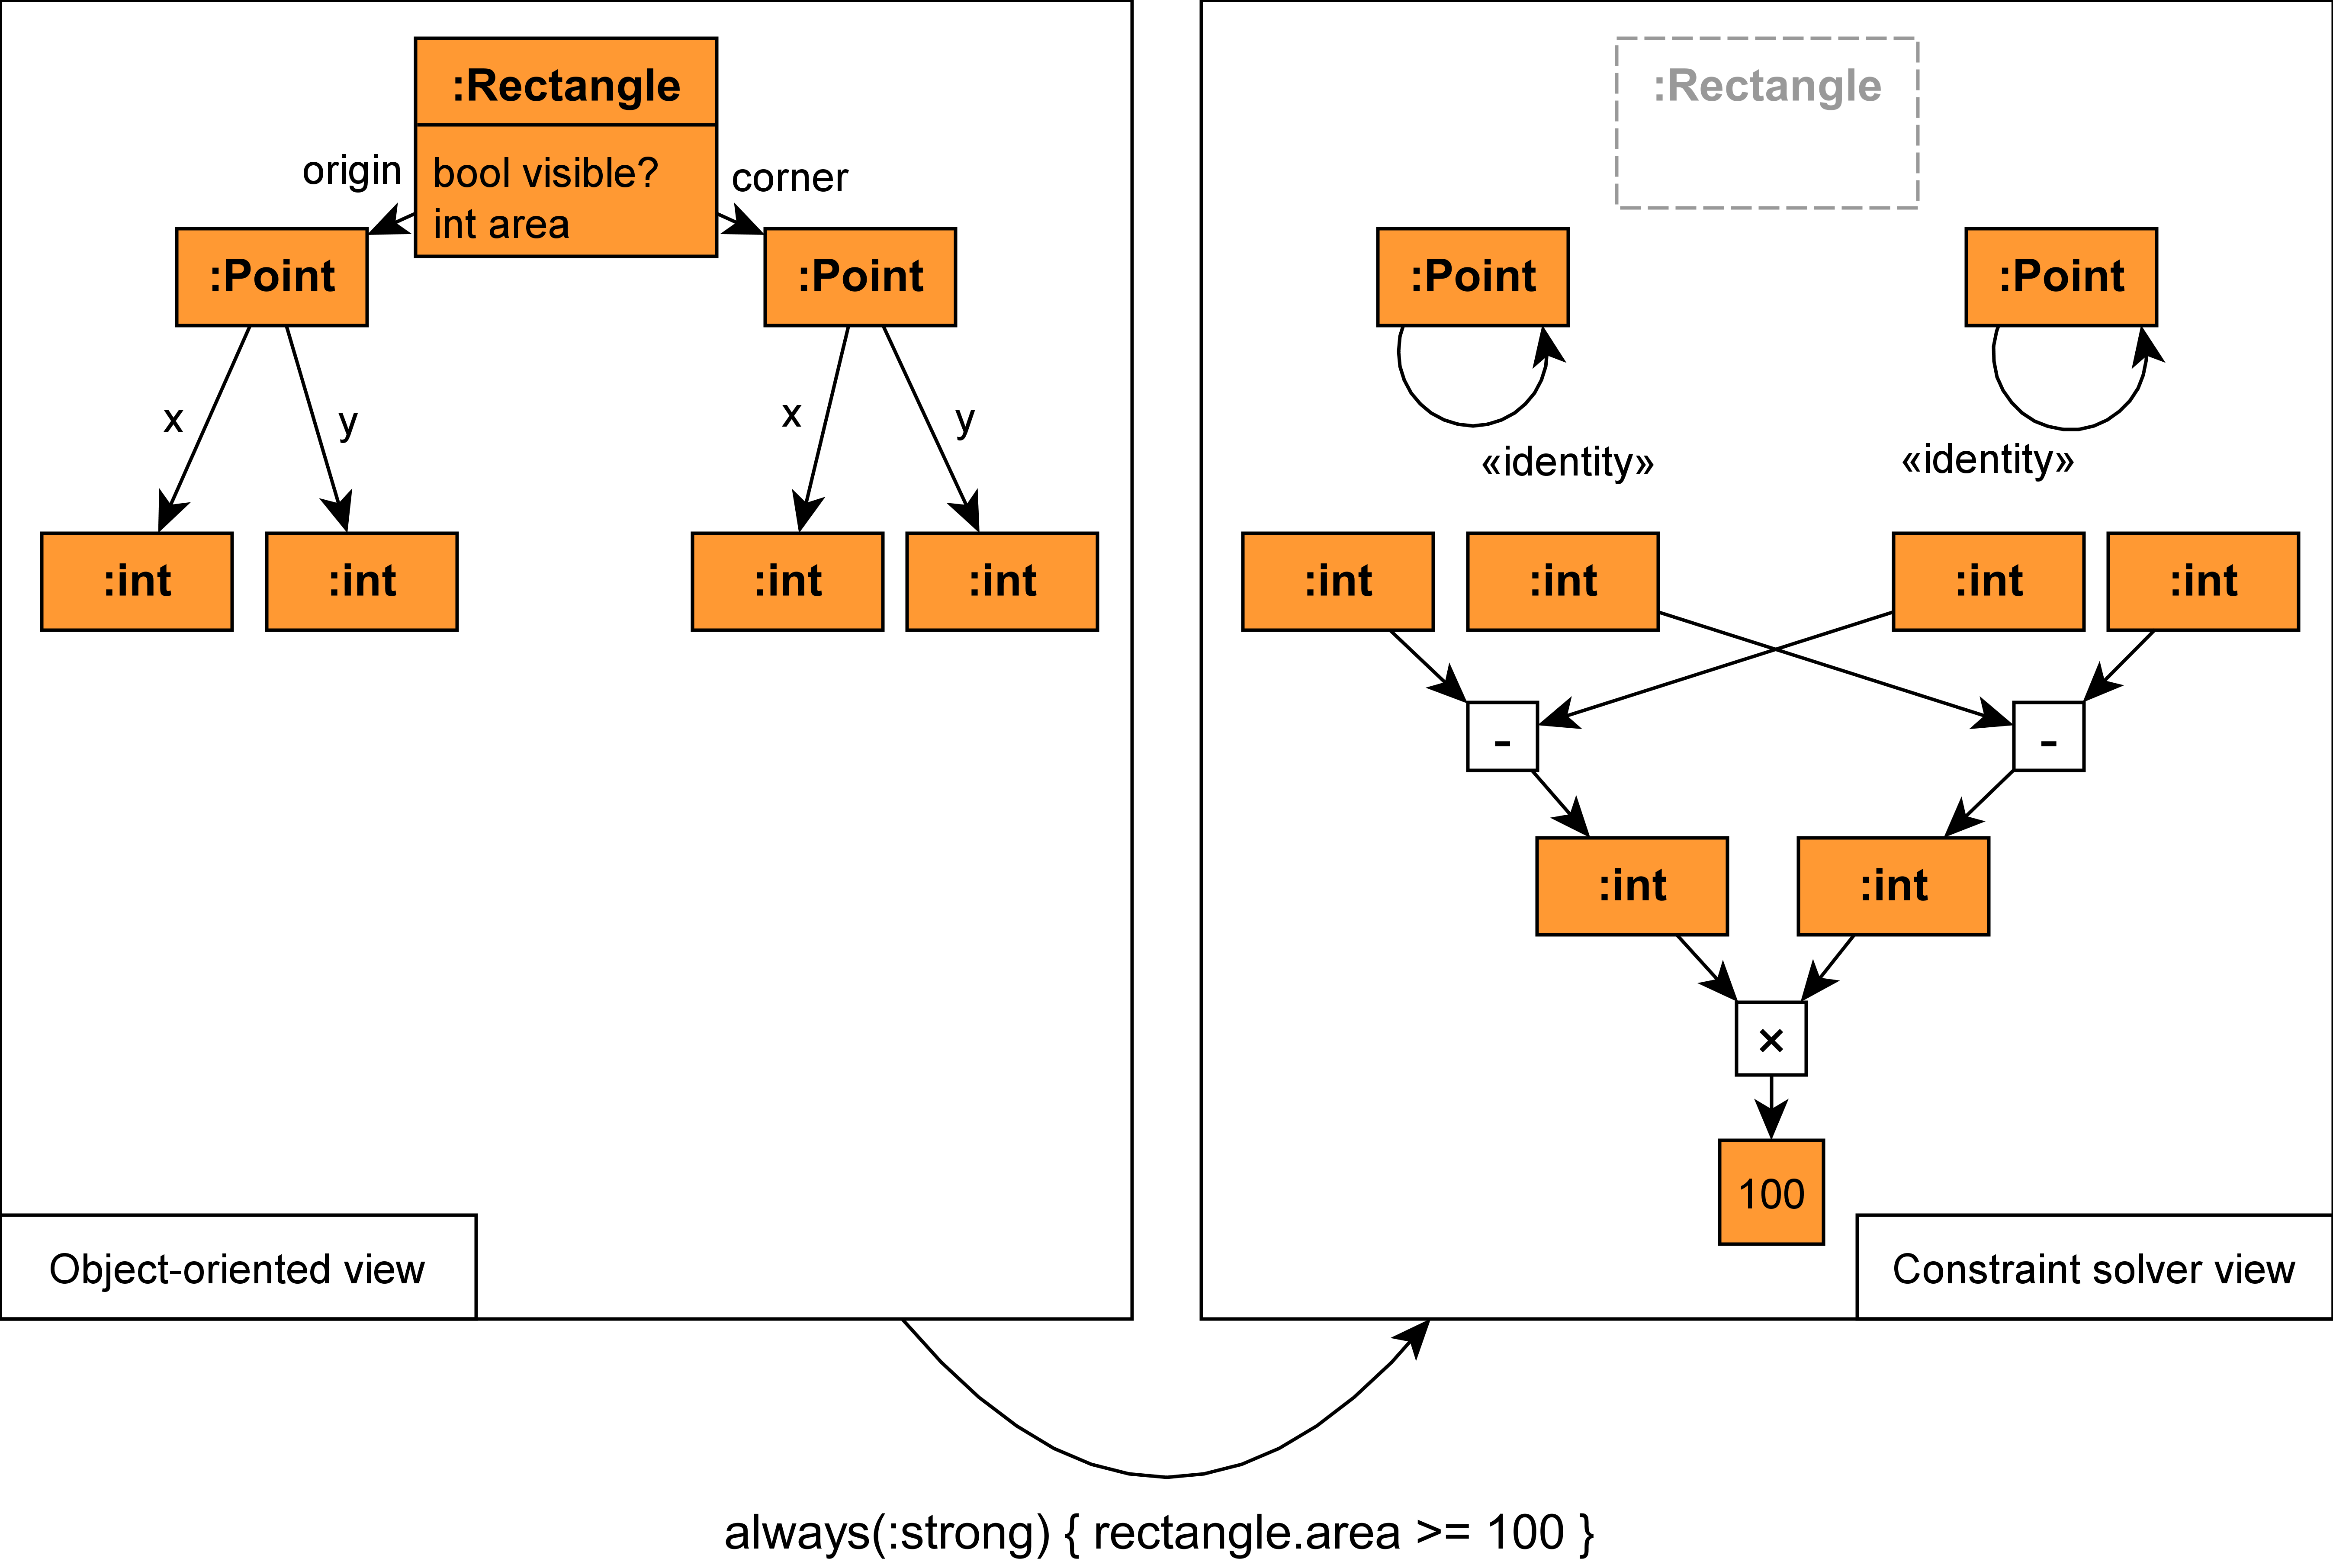
\includegraphics[width=\linewidth]{architecture}
  \caption{Objects are connected through instance variables. When a
    constraint is constructed, objects become connected through
    constraints as well}
\label{fig:architecture}
\end{figure}

The constraint construction is complete when block passed to
\lstinline{always} returns. Any constraint values and combinations
thereof created during the execution are gathered into a
\emph{Constraint}. These provide a meta-level interface to enable or
disable the entire constraint (and thus all participating values),
query and change its priority
(\cf {\autoref{sec:methods-class-constraint}}), and access the block that
was passed to \lstinline{always}, as well as each constraint value that
participates in the constraint.

The constraint then includes a) primitive values that are in the type
domain of the solver and are connected in a constrainable way (\eg
through equalities or inequalities, arithmetic, boolean logic) and b)
a number of marked values for complex objects that invalidate the
constraint if their identity changes.

The constraint solvers operate on primitive constraint values directly
to solve the constraint. Changes made by the solver to the variables
show up in the \ac{oo} view on the next access to the variables from
imperative code, at which point the constraint values are copied to
their \ac{oo} counterparts. Assignments to any variable encountered
during the constraint construction will trigger the solver to
re-satisfy the constraint (and potentially raise an error if the
assignment is inconsistent with the constraint).

Placeholder constraint values invalidate the constraint if the
identity of the \ac{oo} value changes through imperative
assignment. This invalidation retracts all constraint values created
during constraint construction and re-executes the block to create new
constraint values. This means that the block may be re-executed
multiple times during the run-time of the program, and any side-effects
should be benign (\cf {\autoref{sec:constraint-restrictions}}).

\subsection{Implementing Edit Constraints}
\label{sec:implementing-edit-constraints}

Edit constraints are used to support incremental constraint
satisfaction, and are important to achieve good performance in
interactive applications.  The \lstinline{edit} method adds an edit
constraint on the edit variables that are in the block, and then
repeatedly calls the solver's \lstinline{suggest_value} method with
each new value from the stream.  When the stream is empty, it removes
the edit constraint and returns.  The priority defaults to the
highest non-required one.  (If \lstinline{:required} is used,
the system raises an exception if the new edit value can't be used.)
Note that this works if the stream is being fed from another process
that provides new values only when available --- the process that has
the edit constraint should just block until one is available.

\langname does not support edit constraints at a language level.
Instead, the definition of the edit method is part of the Cassowary
solver library that is included in the current version of
\toolname. The library uses the \ac{api} of the \lstinline{Constraint}
class to access the constraint values associated with variable names,
creates edit constraints for them, and feeds the stream into the
resulting edit variables.

Cassowary as shipped in the \toolname standard library allows the
variables and stream to hold user-defined objects, not just primitive
types. To use Cassowary as the solver, we need to convert these into
edit constraints on Floats or other primitive objects (\eg the x and y
values of the midpoint), but we also want to do this in an
object-oriented way that respects encapsulation.  Further, updating
the solution with each new value should continue to be very fast.

To support this, the client passes an array of accessor method names
for the return values that should be updated in the edit
constraint. Cassowary internally creates external variables that it
uses as edit variables. Those external variables are equality
constrained to the return values of the accessor methods, so the
internal storage layout of the class does not matter. In the following
example, mouse locations or the mouse point may be arc points or store
x and y values directly, the edit constraints work simply on the
return values of their respective x and y methods:
\begin{code}
edit(stream: mouse.locations.each,
     accessor: [:x, :y]) { mouse_point }
\end{code}

For DeltaBlue, the edit constraints returned could be simpler, \eg the
point would be simply updated rather than dealing with its x and y
coordinates separately.

\subsection{Adding new Solvers}
\label{sec:solver-interface}

During constraint construction, the \ac{vm} sends
\lstinline{for_constraint} to each variable encountered during the
execution. User code can add solvers to the system by adding a
\lstinline{for_constraint} method to those classes that the solver can
work with, making use of Ruby's open classes. This method takes the
name under which the variable is accessed as argument, and should
return an object that implements a subset of the interfaces
that the solver can reason about. For Cassowary, we extended the Float
class:
\begin{code}
  def for_constraint(name)
    v = Cassowary::Variable.new(name: name, value: self)
    Cassowary::SimplexSolver.instance.add_stay(v)
    v
  end
\end{code}

This method creates a new variable, adds a low-priority stay so the solver
attempts to keep the value stable, and returns the constraint
object. The \ac{vm} then sends messages to this object instead of the
Float object in the context of the constraint execution.

We expect the objects returned from a \lstinline{for_constraint}
method to respond to two messages:
\begin{description}
\item[suggest\_value] When imperative code stores into a variable that
  participates in constraints, the \ac{vm} instead sends this message
  to the associated constraint object. This method triggers the
  solver, raising an exception if a required constraint can no longer
  be satisfied.
\item[value] Whenever the \ac{vm} accesses a variable that
  participates in a constraint, it sends this message to the
  associated constraint object to determine whether the variable was
  updated by the solver.
\end{description}

In the case of immutable objects (such as floats and integers), the
\ac{vm} updates the reference for the variable directly. However, for
mutable objects, solver libraries should provide the method
\lstinline{assign_constraint_value} to update the object. We provide
such a method for the Array class, which replaces the array's contents
with the contents suggested by the solver:
\begin{code}
  def assign_constraint_value(new_ary)
    self.replace(new_ary)
  end
\end{code}

This illustrates how the solvers provided by \toolname are simply
constraint solver libraries that extend core classes.

%% If we have a subsection on solver interface implementation:
% 
% As far as Cassowary is concerned, a read-only variable is just a
% constant (or an edit variable if it is to be changed repeatedly).


\section{Evaluation}
\label{sec:evaluation}
We evaluate \langname and \toolname first with respect to performance,
and second with respect to how well the language supports desirable
semantic properties for an object constraint language.

\subsection{Performance Evaluation}
\label{sec:performance-evaluation}

There are three questions we are interested in regarding performance:
a) how does constraint solving performance compare to writing
imperative code to satisfy constraints, b) how is object-oriented
performance affected by our extensions to the \ac{vm}, and c)
how does a practical application perform if refactored to use
constraints.

\paragraph{Constraint Solving}
To answer the first question, we used an example from
\cite{lopez-asi-1994} and adapted it to \toolname. In this example,
the user drags the upper end of the mercury in a thermometer using the
mouse. However, the mercury cannot go outside the bounds of the
thermometer, even if the user tries to drag it out. Additionally, a
gray and white rectangle on the screen should be updated to reflect
the new mercury position, and a displayed number should reflect the
integer value of the mercury top.

\begin{figure}[h!]
  \begin{subfigure}[b]{0.48\textwidth}
    \begin{code}[basicstyle=\scriptsize,frame=none]
Iterations.times do |i|
  mouse.location_y = i
  old = mercury.top
  mercury.top = mouse.location_y
  if mercury.top > thermometer.top
    mercury.top = thermometer.top
  end
  temperature = mercury.height
  if old < mercury.top
    # moves upwards (draws over the white)
    gray.top = mercury.top
  else
    # moves downwards (draws over the gray)
    white.bottom = mercury.top
  end
  display.number = temperature
end
    \end{code}
    \caption{Imperative version}
  \end{subfigure}
  \begin{subfigure}[b]{0.52\textwidth}
    \centering
    \begin{code}[basicstyle=\scriptsize,frame=none]
always { temperature == mercury.height }
always { white.top == thermometer.top }
always { white.bottom == mercury.top }
always { gray.top == mercury.top }
always { gray.bottom == mercury.bottom }
always { display.number == temperature }
always(:high) { mercury.top == mouse.location_y }
always { mercury.top <= thermometer.top }
always { mercury.bottom == thermometer.bottom }
always { thermometer.bottom == 0 }
always { thermometer.top == 200 }

Iterations.times do |i|
  mouse.location_y = i
end
# edit(Iterations.times) { mouse.location_y }
    \end{code}
    \caption{Object-constraint version}
  \end{subfigure}
  \caption{Interactive thermometer example from \cite{lopez-asi-1994}}
  \label{fig:thermometer-example}
\end{figure}

Note that the object-constraint version may be written in two ways:
one that is more like the imperative version and assigns new mouse
locations in a loop; and a more constraint-oriented version that
declares \lstinline{mouse.location_y} as an edit variable that
triggers incrementally re-satisfying the constraints. In our benchmarks
we have run both variants.

\begin{table}
  \centering
  \begin{tabular}[h]{r|c c c}
    Iterations & Imperative & Constraints & Edit Constraints \\
    \hline
    100 & 1($\sigma$0.241) & 36.1($\sigma$3.14) & 6.24($\sigma$0.828) \\
    10,000 & 1($\sigma$0.14) & 629($\sigma$6.91) & 7.72($\sigma$0.526) \\
    1,000,000 & 1($\sigma$0.12) & 45137($\sigma$458) & 52.5($\sigma$2.24) \\
  \end{tabular}
  \caption{Thermometer benchmark (normalized against imperative version)}
  \label{fig:thermometer-benchmark}    
\end{table}

% \begin{figure}
%   \begin{subfigure}[c]{0.45\textwidth}
%     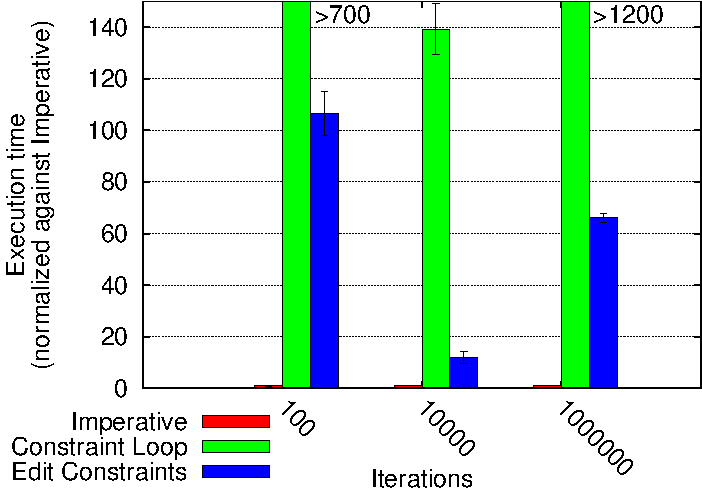
\includegraphics[width=\textwidth]{thermometer.pdf}
%   \end{subfigure}
%   \begin{subfigure}[c]{0.45\textwidth}
%     \centering
%     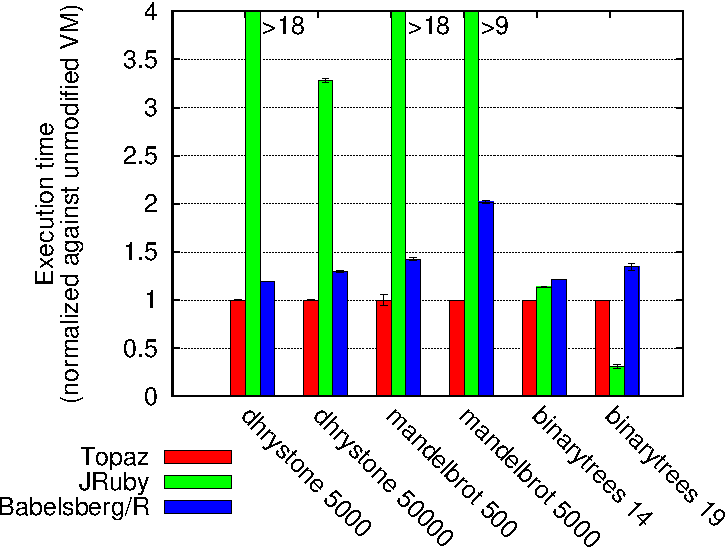
\includegraphics[width=0.6\textwidth]{metatracing_vms_benchmarks.pdf}
%     \caption{Metatracing \acp{vm} benchmark}
%     \label{fig:metatracing-benchmark}    
%   \end{subfigure}
%   \caption{Benchmarks for constraint solving and imperative code
%     execution, run on an Intel i7 Quad-Core CPU with 3.4 GHz}
% \end{figure}

\autoref{fig:thermometer-benchmark} shows that the naive
object-constraint version is usually many hundred times slower than
the purely imperative solution. As the iteration count grows, the
naive version also does not seem to benefit as much from the \ac{jit}
as the imperative version. Using edit constraints, repeated solving of
constraints is much faster. Keep in mind that these results use a
solver that is also written in pure Ruby, which is by itself orders of
magnitude slower than a C++ based version. Considering that \toolname
is aimed at imperative programmers, we expect that most of the time
the \ac{vm} will not be solving constraints in tight loops, but
running mostly imperative code intermingled with constraint
re-satisfaction.

\paragraph{Object-oriented Performance}

For imperative code performance, we ran a number of tests from the
metatracing \acp{vm} experiment~\cite{bolz2013impact} against the
unmodified \emph{Topaz} Ruby \ac{vm} and the \emph{JRuby} \ac{vm}.

\begin{figure}
  \centering
  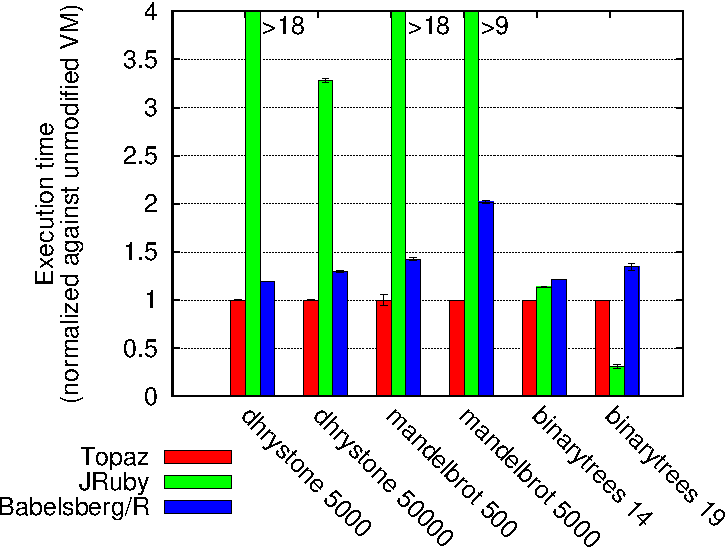
\includegraphics[width=0.6\textwidth]{metatracing_vms_benchmarks.pdf}
  \caption{Metatracing \textsc{vm} benchmark run on an Intel i7 Quad-Core
    CPU with 3.4 GHz}
  \label{fig:metatracing-benchmark}    
\end{figure}
%% \ac{vm} in the \caption didn't work -- removed

For purely imperative code, \toolname is consistently less 1.5 times
slower in these benchmarks than the unmodified \ac{vm}
(\autoref{fig:metatracing-benchmark}). The only benchmark where we are
doing significantly worse than Topaz is
\emph{Binarytrees}. Binarytrees is a strongly recursive benchmark,
which Topaz' (and thus \toolname's \ac{jit}) is bad at optimizing
(which is why JRuby does better in this benchmark). The overhead in
\toolname is mostly due an additional test each time a variable is
accessed, to check whether this variable participates in a
constraint. An annotation in the \ac{vm}~\cite{bolz2011runtime} allows
the \ac{jit} to remove this test when there are no constraints on
variables in the loop, but in \emph{Binarytrees}, we do not generate
machine code for a large part of the code (due to its recursive
nature), and the test incurs some overhead.

Considering that JRuby and Topaz are, for these benchmarks, currently
the fastest Ruby \acp{vm}, we consider \toolname to be very performant
for purely imperative code.  

\paragraph{Application Example}
We have written a simple video streaming application. This application
reads a folder with bitmaps and streams raw video to a video
player. The quality with which the video is streamed depends on a
number of variables:
\begin{description}
\item[User Preference] Users may decide not to overload their systems
  and explicitly choose a lower quality. This should be an upper
  bound for the quality of the streaming.
\item[Encoding Time] The program has only 1/25 second to encode a
  frame. If it takes longer, the quality should be automatically
  reduced to ensure smooth playback.
\item[System Load] The overall system load of the encoding system
  should be less than 80\%, to retain enough resources for other tasks.
\item[Quality Bounds] Whatever users choose as preferred quality, the
  quality cannot be below 0 or above 100\%.
\end{description}

In the imperative version of the application, these constraints were
explicitly checked and re-satisfied after each frame. The
object-constraint solution uses custom solvers for File contents and
method execution time:
\begin{figure}[h!]
  \begin{subfigure}[b]{0.48\textwidth}
    \begin{code}[basicstyle=\scriptsize,frame=none]
def recalculate_quality
  if @quality + encoding_time < 90
    @quality = @quality + encoding_time
  elsif @quality + encoding_time > 100 + FrameMsMax
    @quality = 100 + FrameMsMax
  end

  if cpuload > 0.8 * NumberOfProcessors
    diff = 100 * (NumberOfProcessors - cpuload)
    if diff > 0
      @quality -= diff
    else
      @quality += diff
    end
  end

  if @quality > user_preference
    @quality = user_preference
  end
  @quality = 0 if @quality < 0
  @quality = 100 if @quality > 100
end
    \end{code}
    \caption{Imperative version}
  \end{subfigure}
  \begin{subfigure}[b]{0.52\textwidth}
    \centering
    \begin{code}[basicstyle=\scriptsize,frame=none]
always { @quality >= 0 }
always { @quality <= 100 }
always { @quality <= user_preference }
always(:high) { @quality == user_preference }
always { @quality + cpuload * 100 <=
             100 + 80 * NumberOfProcessors }
always(:high) { @quality + encoding_time >= 90 }
always { @quality + encoding_time <=
             100 + FrameMsMax }
    \end{code}
    \caption{Object-constraint version}
  \end{subfigure}
  \caption{Quality constraints in video streaming}
  \label{fig:video-streaming-example}
\end{figure}

Both versions could stream video at the highest quality setting to up
to 8 clients on an Intel i5 2.4 GHz CPU. Both reduced the quality
afterwards. Because most of the time was spent encoding and streaming
video, both versions performed equivalently well.

%% \ac{vm} in the \paragraph{....} title didn't work -- changed to
%% just use capitals
\paragraph{VM Hooks for Customizing Constraint Construction}
The \ac{vm} hook methods \lstinline{for_constraint} and
\lstinline{assign_constraint_value} are useful not only for solvers,
but also if users want to provide a particular interpretation of
certain application domain objects in their constraints. In
\autoref{fig:video-streaming-example} we use the contents of a
preference file and the last execution time of the frame encoding
method in our constraints.

The effort to allow Cassowary to work with file content and method
execution time was minimal. The following class definition was enough
for us to be able to use the execution time of a method in a
constraint:
\begin{code}
class MethodTimer
  def initialize(klass, symbol)
    time = 0
    @constrained_time = Constraint.new { time }

    old_method = klass.instance_method(symbol)
    klass.define_method(symbol) do |*args, &block|
      start = Time.now
      res = old_method.bind(self).call(*args, &block)
      time = Time.now - start
      res
    end
  end

  def for_constraint(name)
    @constrained_time.?
  end
end
\end{code}

A \lstinline{MethodTimer} can be instantiated with a class and the
name of a method, and wraps this method to record its last execution
time. When used in a constraint, a read-only constraint object is
returned that was associated with the \lstinline{time} local
variable. Because it is read-only, the
\lstinline{assign_constraint_value} method is omitted. For the
configuration file object, the \lstinline{assign_constraint_value}
method is as follows:
\begin{code}
  def assign_constraint_value(float)
    if float != @content.to_f
      raise "cannot assign to read-only file" unless @writable
      @file.truncate(0)
      @file.rewind
      @file.write(float)
    end
  end
\end{code}

This illustrates that our \ac{vm} hooks for constraint construction
provide a limited local propagation mechanism to interpret complex
objects in the type domain of a particular solver.

\subsection{Comparison with Related Approaches}
\label{sec:comparison}

\langname has a number of properties that we think are desirable for
an object-constraint programming
language. \autoref{tab:cmp-constraint-lang-approaches} shows these
properties and compares \ac{ocp} to related approaches presented in
\autoref{sec:background-related-work}.  As a continuation of
\ac{cip}, \ac{ocp} shares most properties with the languages like
Kaleidoscope and Turtle.

\begin{table*}
  \centering
  \begin{tabular}{l|c|c|c|c|c}
    & Libraries & \textsc{dsl} & Dataflow/\textsc{frp} & \textsc{cip} & \textsc{ocp} \\
    Unified Language Constructs & & & & & x \\
    Automatic Solving & & x & x & x & x \\
    Linguistic Symbiosis & & & x & x & x \\
    Extensible Solvers & x & & (x) & (x) & x \\
    Suitably Expressive Constraints & x & x & & x & x \\
    Performant Pure-\ac{oo} code & x & x & x & & x \\
  \end{tabular}
  \caption{Comparison of OCP with related work}
  \label{tab:cmp-constraint-lang-approaches}
\end{table*}

\paragraph{Unified Language Constructs}
Programs in \langname appear as ordinary \ac{oo} programs if no
constraints are used, but can be easily adapted to use constraints
where it makes sense. If constraints are used, they respect
encapsulation and re-use the object-oriented method
definitions. Furthermore,  techniques such as
inheritance and dynamic typing operate correctly with constraints.

In contrast, library and \ac{dsl} based approaches separate
constraints from imperative code through a different syntax and
semantics. For example, \ac{frp} and \ac{cip} languages use
\emph{propagation hooks} and \emph{constraint constructors}
respectively to support constraints. Here, propagation hooks are the
functions connecting variable that are called when one variable
changes to compute a new value for the downstream variable. Constraint
constructors are the concept in Kaleidoscope to build higher order
constraints. In the simplest case these are rewrite rules to convert
constraints on complex objects into primitive constraints for a
solver. In Kaleidoscope, messages in constraint expressions are
dispatched to constraint constructors using multi method lookup
semantics, where the receiver and all arguments participate in the
method selection.

\paragraph{Automatic Solving}
Using libraries for constraint satisfaction allows programmers to
write code that (intentionally or unintentionally) circumvents
previously asserted constraints. Approaches that integrate constraints
at a language level do not allow such circumvention, and attempt to
re-satisfy constraints whenever they are violated during program
execution.

\paragraph{Linguistic Symbiosis}
D'Hondt et al.~\cite{d2004seamless} argue that linguistic symbiosis
between different programming paradigms is required to support the
evolution of programs from the object-oriented paradigm to a
constraint-oriented solution and vice versa. \ac{dsl} and library
based approaches do not support such incremental refactoring between
paradigms as well as approaches in which constraints are written in the
host language.

\paragraph{Extensible Solvers}
Libraries provide the most flexibility for choosing different solvers
depending on programmer needs. \ac{frp} languages can, to some extent,
be combined with solver libraries to achieve a comparable
flexibility. \ac{cip} languages also provide a more controlled way for
developers to use different solvers by writing constraint constructors
that reformulate constraints using a different solver.

In \langname, all solvers use the same interface to communicate with
the \ac{vm} so developers can add new solvers and replace existing
ones to support new type domains, or to use solvers that give better
results or performance for a particular problem.

\paragraph{Suitably Expressive Constraints}
To take advantage of the constraint paradigm, the language should
allow a rich set of constraints to be written and solved.
Multi-directional constraints are important for some applications,
while others additionally require solvers that can accommodate
simultaneous equations and inequalities.  (For example, the Wheatstone
bridge example requires solving simultaneous equations, while the
video streaming example needs inequalities as well as equalities, and
both hard and soft constraints.)  On the other hand, given an overly
powerful language, it becomes all too easy to write constraints that
take a very long time indeed to solve or that are intractable.  We
believe that \langname strikes an appropriate balance here, by
providing an expressive set of constraints with the solvers in the
initial library, and by allowing more powerful solvers to be added if
desired.  However, much more experience is needed to test whether in
fact this is an appropriate balance, and to adjust it as needed; and
as noted in the ``Conclusion and Future Work'' section, an important
direction will be adding better support for debugging, explanation,
and benchmarking.

\paragraph{Performant Pure OO Code}
Kaleidoscope provided a declarative semantics for assignment, type
declaration, and subclassing. However, this declarative semantics was
also used if no actual constraints are in the program. Our
implementation approach in \toolname uses different execution contexts
for constraint construction/solving and imperative code. Combined with
a state of the art \ac{jit}, this gives performance for pure \ac{oo}
code that is generally comparable to a standard \ac{oo} \ac{vm} as used for
other approaches.

\section{Conclusion and Future Work}
\label{sec:conclusion}
We have presented \langname, an object constraint language that extends
a standard object-oriented language to support constraints, along with
an implementation as an extension to Ruby using a state of the art
virtual machine.  In contrast to other approaches, \langname unifies
the constructs for encapsulation and abstraction for both the
declarative constraint parts of the language and the traditional
imperative parts by using only object-oriented method definitions for
both declarative and imperative code.  Our implementation is
integrated with an existing object-oriented virtual machine, and
provides a standard imperative evaluation mode, a constraint
evaluation mode that accumulates constraints to hand off to the solver
as expressions are evaluated, and a constraint solver mode.

This work is relatively recent and there are a number of directions
for future work.  One is to exercise the system on a wider variety of
programs, and also to work on improving the performance of the
constraint evaluation and satisfaction.  Another direction is to add
additional solvers to the library, for example a finite domain solver
or solvers that support constraints on other primitive storage types
such as arrays, strings, and hashes, and to implement the design for
cooperating solvers.  The multi-assignment semantics described in
\autoref{sec:constraint-durations-and-activation} provides a clean and
simple way to control when constraint satisfaction is invoked.
However, more experience with writing programs in \toolname is needed
to decide whether this construct is sufficiently expressive, or
whether additional ways are needed to control when constraint solving
is invoked.  Yet another direction regarding solvers is to introduce a
``meta-solver'' that can automatically select one or more applicable
solvers for the given set of constraints.

Another important direction will be adding better support for
debugging, explanation, and benchmarking.  (If the constraint solver
is unable to satisfy the constraints, why is this?  Or if the solver
produces an unexpected answer, how was this answer arrived at?  If the
solver is slow, why, and are there ways to make it faster?  Is there a
more appropriate solver available?)

Our initial implementation extends Ruby, but the ideas are applicable
to other dynamic object-oriented languages, and future work may
include versions in Javascript or Squeak. 

% In particular, a constraint extension to Javascript would be of
% particular interest given the potential for integration with Lively.

%% - solves 2 shortcoming of other constraint programming languages
%%   1. preserves encapsulation
%%   2. exchangeable solver, changeable
%%   3. modularized constraints
%% - promising approach to 1 more general problem, that we will investigate
%%   * how to integrate different execution models (declarative, imperative)
%% - good benchmark results show that it can be performant

% LocalWords:  Modularity Lugano Babelsberg hpi nowrap Felgentreff uw Borning
% LocalWords:  Hirschfeld Hasso Plattner articleno doisuffix invariants vm dsl
% LocalWords:  subregion toolkits interoperate superset incrementality resize
% LocalWords:  cryptarithmetic checkable DISPLAYWIDTH DISPLAYHEIGHT attr rect
% LocalWords:  accessor RectAspect args postAdvice dataflow SMT kodkod Aukland
% LocalWords:  DeltaBlue multi CPLEX ctx booleans runtime run-time css Enaml enameldef
% LocalWords:  FRP LivelyKernel Webwerkstatt KScript prevOrigin isVisible CLP
% LocalWords:  prevExtent Siri Samimi Aung Millstein Demsky Rinard mileaux JIT
% LocalWords:  Kaleidoscope'90 Kaleidoscope'93 TemperatureConverter fahrenheit
% LocalWords:  lead1 lead2 boolean disjunctions unsatisfiable 's parameterized
% LocalWords:  desiredsize Durations durations PyPy RPython toolchain RPython's
% LocalWords:  jit globals oo ConstraintInterpreter bytecodes initializer api
% LocalWords:  bytecode subclasses ConstraintObject unevaluated constrainable
% LocalWords:  equalities ary refactored basicstyle Metatracing i7 Ghz elsif i5
% LocalWords:  metatracing performant FrameMsMax FrameTime cpuload MethodTimer
% LocalWords:  NumberOfProcessors klass Ghz frp cip ocp Smalltalk inlines Z3 's
% LocalWords:  lookup subclassing Ghz Ghz Ghz FRAGE sind da nicht richtig drin
% LocalWords:  erwaehnen Prolog benchmarking Javascript Javascript DOIs ACKS p1
% LocalWords:  von Sternberg's acyclic SkyBlue iff CartesianPoint tex Z3Asts r1
% LocalWords:  LinearEqualities stringA stringB pt1 pt2 TwoLeadedObject r2 r3
% LocalWords:  wheatstone r4 ListCell DoublyLinkedListCell prev TODO  's 's cmp
% LocalWords:  Javascript multiobjective optimizations BackTalk impl JRuby lang
% LocalWords:  Binarytrees Topaz' D'Hondt et al versa refactoring Javascript
% LocalWords:  alldifferent

%%% Local Variables: 
%%% mode: latex
%%% TeX-master: "babelsberg_jot"
%%% End: 


\subsection*{Acknowledgments}
\begin{quotation}
  \noindent I owe everything to my ``Mäuschen''.
\end{quotation}

%%% Local Variables:
%%% mode: latex
%%% TeX-master: "Felgentreff_2014_Babelsberg"
%%% End:


\backmatter
\bibliographystyle{plain}
\bibliography{qiqqa_jot_export,constraints,sigproc}

\newpage
\appendix
\lstset{basicstyle=\footnotesize\ttfamily}
\section{Appendix}

This appendix contains material not published in the journal article,
including a design for additional language features not yet
implemented, and example programs.  All the example programs are fully
functional with the current implementation.

\subsection{About the Name}

%% \begin{wrapfigure}{r}{0.25\textwidth}
%%   \begin{center}
%%     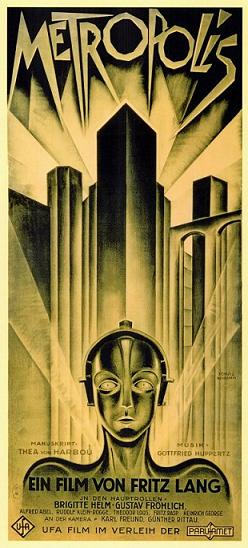
\includegraphics[width=0.25\textwidth]{Metropolisposter}
%%   \end{center}
%% \end{wrapfigure}

Babelsberg is a district of Potsdam, in which HPI is located.  It is
also the location of Studio Babelsberg, the historical center of the
German film industry (Fritz Lang's \emph{Metropolis} and Josef von
Sternberg's \emph{The Blue Angel} were filmed there), and still
active, primarily for high-budget feature films.

% \begin{figure}[h]
%   \begin{center}
%   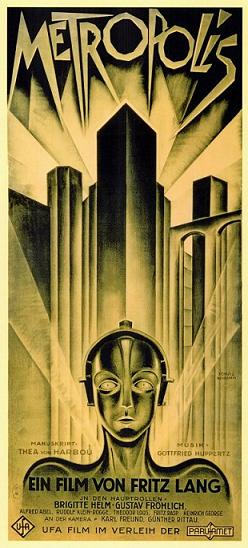
\includegraphics[width=0.25\textwidth]{Metropolisposter}
%   \end{center}
%   \caption{Poster for ``Metropolis''}
% \end{figure}

\subsection{Support for Multiple Cooperating Solvers}
\label{sec:cooperating-solvers}

The current implementation supports multiple solvers, and a protocol
for solvers so that it is convenient to add new ones.  However, for a
given variable only one solver is used.  This is a significant
limitation, since richer sets of constraints can be written and solved
using multiple cooperating solvers.  The Viewpoints note
``Architectures for Cooperating Constraint Solvers''
\cite{borning-coop-solvers-2012} describes one technique for
supporting this, which fits well with \langname.
%% Our more recent
%% work with Bloom as an infrastructure for cooperating solvers takes a
%% more general approach, which will also be more complex to implement.
%% We suggest an evolutionary path for \langname that begins with the
%% former approach, and perhaps later encompasses the Bloom approach.
Briefly, in the ``Architectures for Cooperating Constraint Solvers''
approach, we view the constraints and constrained variables as a
bipartite graph.  For the top level, we partition the constraints into
regions, based on the following requirements:
\begin{itemize}
\item each constraint belongs to exactly one region
\item the different regions can share variables (but not constraints)
\item for each variable shared by two or more regions, that variable
  must be read-only for all but one of the regions
\item the graph of the different top-level regions must be acyclic
\item it isn't possible to divide any region into two regions and
  still maintain the other requirements
\end{itemize}

We can always partition the constraint graph this way.  (In the limit,
there is a single region.)  The partitioning is unique.

Given this partitioning, and a solver for the constraints in each
region, it is easy to solve the constraint system as a whole: it is just
a dataflow problem.  We find an order for solving the regions, so that
region B is solved after region A if B is downstream from A in terms
of the read-only variables.

%% merge any of this material that's still relevant into the next
%% section

%% \subsection{Support for Local Propagation Constraints and Solvers}

%% Local propagation solvers are useful since they are efficient and can
%% be used with constraints on arbitrary kinds of values.  They have
%% important limitations as well --- in particular they don't handle
%% simultaneous equations, or constraints that don't uniquely determine
%% values for the constrained variables, such as inequalities.  We
%% believe that it is important to support them in \toolname, and also
%% that they be part of a suite of cooperating solvers, others of which
%% \emph{can} handle such kinds of constraints.

%% To allow a constraint to be used with a local propagation solver, the
%% programmer should supply a set of \emph{constraint methods}, one for
%% each writable variable (\ie a variable referenced by the constraint
%% that isn't read-only).  Evaluating the method should set the
%% corresponding variable to a value that satisfies the constraint.  The
%% constraint should be functional for each of its writable variables,
%% \ie the value for that variable should be unique given values for
%% the other constrained variables.  If a constraint is read-only in some
%% variable, then it doesn't need a method for that
%% variable.\footnote{Prior work has sought to remove the restriction
%%   that the local propagation constraint be functional in the writable
%%   variables, so that for example one can use inequalities with local
%%   propagation.  Other work has included local propagation constraints
%%   whose methods set more than one variable (\eg SkyBlue).  However,
%%   these solvers are more difficult for the programmer using them to
%%   understand, so we use basic version of local propagation here.  Note
%%   that if there is only one method per constraint, with all of the
%%   other constrained variables being read-only, local propagation
%%   reduces to dataflow constraints.}

\subsection{Initializing and Manipulating Constraints}
\label{sec:initializing-constraints}

This subsection describes the protocol for initializing constraints
and the methods available on constraint objects.

Formally, a constraint is just a predicate that we want to have hold.
In the implementation, it is represented as an instance of
\lstinline{Constraint}.  Minimally, a constraint can be defined just
as a predicate, written as a Ruby block.  The block should meet the
following criteria:

\begin{itemize}

\item Evaluating the block returns a boolean --- the constraint is
  that it evaluate to true.

\item The expression in the block should either be free of side
  effects, or if there are side effects, they should be benign (for
  example, doing caching).  

\item Repeatedly evaluating the block should return the same thing (so
  an expression involving a random number generator wouldn't qualify).

\end{itemize}

There should be other available attributes for
\lstinline{Constraint}.  Constraints that will be satisfied
using a local propagation solver need a set of propagation methods,
soft constraints need a priority, and so forth.  

\subsubsection{The Syntax of the always Primitive }
\label{sec:synt-always-prim}
The syntax for the \lstinline{always}
primitive is the same as for a normal method
call, but is given here to document the interpretation of the
arguments. Note that the \lstinline{SOLVER_SPECIFIC_ARGS} rule only
gives examples, and different solver libraries can accept different
optional arguments here, but should have sane defaults, if none are
given. The definition of \lstinline{RUBY_STATEMENT} is omitted
(\cf{\cite{flanagan2008ruby}}).
\begin{lstlisting}{columns=fixed}
ALWAYS: "always" ["(" ALWAYS_ARGS ")"] CONSTRAINT_BLOCK

ALWAYS_ARGS: ["solver:" RUBY_STATEMENT] [SOLVER_SPECIFIC_ARGS]
            | [SOLVER_SPECIFIC_ARGS]

SOLVER_SPECIFIC_ARGS: ["priority": PRIORITY] [SOLVER_ARGS]
                      | [predicate": BLOCK] [SOLVER_ARGS]
                      | // ...

PRIORITY: "required" | "high | "medium" | "low"

CONSTRAINT_BLOCK: "DO" RUBY_STATEMENT* "END"
                  | "{" RUBY_STATEMENT* "}"
\end{lstlisting}

\subsubsection{Initializing a Constraint}

Here is a list of attributes that can be supplied when initializing a
constraint object.  The predicate is the only required one, and as
described below can be either an argument or a block after the
arguments.  All of the other attributes are specifiable as optional
arguments to \lstinline{always} or \lstinline{once}.

\begin{description}
\item[predicate] A block that evaluates to true or false.  
\item[priority] Defaults to \lstinline{:required}.
\item[weight] Defaults to 1.
\item[error] A block that evaluates to the error in satisfying that
  constraint.  The error value is 0 iff the constraint is satisfied.
  Defaults to a simple 0/1 function.
\item[methods] (optional) A dictionary of local propagation methods, indexed by
  the variable whose value is computed by the corresponding
  method.
\end{description}

The local propagation methods are only needed for local propagation
solvers such as DeltaBlue.  Each method is a block, that if evaluated,
will set the index variable to a value that satisfies the constraint.
The constraint should be functional for the writable variables, \ie
the value for the index variable should be unique given values for the
other constrained variables.  If a constraint is read-only in some
variable, then there isn't a corresponding block for that variable in
the dictionary.

\lstinline{always} can be used to define compound constraints. This
happens, for example, if a predicate method checks two conditions and
conjoins them (as, for example, in a \lstinline{CartesianPoint#==}
method).  All arguments apply to all constraint parts that are created
during the execution of \lstinline{always}. So a \lstinline{:low} priority
compound constraint will be added to the solver as multiple primitive
constraints that are all \lstinline{:low} priority.  If local propagation
methods are provided, evaluating a method must satisfy all of the
component constraints of a compound constraint.  The error for a
compound constraint is likely to be problematic unless it is a simple
0/1 function.

%% TODO: fix the discussion of local propagation methods, to account
%% for the current syntax

%% Here's a trivial example for the $x+y=z$ constraint.  

\subsubsection{Methods for the Class Constraint}
\label{sec:methods-class-constraint}

The \lstinline{Constraint} class provides the following methods in
\toolname.  (Here we are referring to ordinary Ruby methods provided
by the class, not the constraint methods for local propagation.)

\begin{description}
\item[enable] Enable all constraints that were asserted in the block.
  (If the constraint is a compound constraint added
  to the solver as multiple primitive constraints, all of these
  primitive constraints are enabled.)
\item[disable] Disable all constraints that were asserted in the block.
\item[priority] Returns the constraint block priority.
\item[priority=] Setter for the constraint block priority. This
  retracts all constraints and re-enables them using the new priority.
\item[constraint\_block] Returns the block object that was passed to
  \lstinline{always}.
\item[solver\_constraints] Returns an array with the solver-specific
  constraint objects. For Cassowary constraints, this is a list of
  \lstinline{LinearEqualities}; for \zthree it is a list of
  \lstinline{Z3Asts}.
\end{description}

\subsection{Constraint Durations}
\label{sec:constraint-durations}

A constraint may not necessarily be active for the entire life of the
program.  \langname provides the following options:
\lstinline{always}, \lstinline{once}, and
\lstinline{assert during} (for constraints that are enforced
while a block is executing and then removed).


The return value of a call to \lstinline{always} is an object of type
\lstinline{Constraint}. If the constraint has no solver, but the
expression already evaluates to true, a warning is printed; if it is
false, an exception is raised.

Currently, all assertions that we want to continuously check,
but cannot yet solve, are implemented in this way. For example, without
enabling any string solvers in the system, 
\lstinline!always { stringA == stringB }! will return \lstinline{true} 
if indeed the two strings
are equal, and whenever either of the strings is assigned, the block is
re-executed to check if the condition still holds. If it doesn't,
an exception is raised.

This same mechanism is used when complex objects for which we have no
solver occur in the constraint expression (even if a primitive
constraint is created in the block). Consider equality between two
Cartesian points, \lstinline{pt1} and \lstinline{pt2}: the constraint
expression will create two primitive constraints, namely that
\lstinline{pt1.x == pt2.x} and \lstinline{pt1.y == pt2.y}. Whenever an
\lstinline{@x} or a \lstinline{@y} of either \lstinline{p1} or
\lstinline{pt2} is assigned, the constraint solver will just calculate
new values for the other instance variables. However, if
\lstinline{pt1} is assigned a new object, the two primitive
constraints are removed from the solver and the constraint block is
executed again, to generate new primitive constraints that 
are equivalent to \lstinline{pt1.x == pt2.x}.
Because \lstinline{pt1} may now be an instance of
a different class, the equality may
be expressed differently. So whenever a complex object occurs in the
execution of a constraint expression, the entire block is retained
as long as the object is, so that the block can be re-executed later
when the object is assigned a new value.

\subsection{Constraint Priorities}

All arguments to \lstinline{always} (except for the block), are simply
passed on to the \lstinline{enable} method of the solver specific
primitive constraint objects asserted during the execution of the
block. \toolname does not have specific constraint priorities built in
(or weights, local propagation methods, or anything else that a particular
solver may use). DeltaBlue and Cassowary---the two solvers that we
currently provide that support priorities---simply map a set of named
priorities to internal priority values: \lstinline{required},
\lstinline{high}, \lstinline{medium}, and \lstinline{low}. 
We currently require that all the solver libraries use the same
priority names.  (Adding a more general mechanism that allows
arbitrarily many priorities, and different names in different
libraries, is a possible extension.  However, in practice we've found
that the fixed set of priorities has been sufficient, because the priorities
tend to be used in stylized ways, \eg \lstinline{high} for edit
constraints and \lstinline{low} for stays.)

%% COMMENTED OUT SINCE NOW MOSTLY REDUNDANT WITH THE CONCLUSION:
%%
%% \subsection{Extending Other Languages}
%% \label{sec:other-languages}

%% \toolname is an extension to Ruby, and Ruby programs without
%% constraints continue to be legal in it.  The Babelsberg syntax takes
%% advantage of some Ruby quirks to provide a convenient syntax, and the
%% implementation (\autoref{sec:implementation}) relies on Topaz, an
%% experimental \ac{vm} built using the PyPy/RPython toolchain.

%% However, the ideas are applicable to other dynamic object-oriented
%% languages, and future work may include versions in Javascript or
%% Squeak.  In particular, a constraint extension to Javascript would be
%% of particular interest given the potential for integration with
%% Lively.

%% Another potential direction for future work is to evolve this language
%% extension to work with the constraint-based extension to Bloom,
%% initially in Ruby, and later in other languages as well to support
%% cooperating languages with constraints.

\subsection{Example Programs}

This part of the appendix provides a set of example programs in
\toolname that illustrate various features of the language.

\subsubsection{Electrical Circuit Examples}
\label{sec:electrical-circuits}

Here is a complete listing of the classes for building simple
electrical circuits with batteries, resistors, wires, and grounds,
along with some sample circuits using them.  Note in particular the
clean way constraints such as Ohm's Law can be expressed, and the
integration of constraints with control structures for the Kirchhoff's
Law constraint that the currents in a list of connected leads sum to 0
in line 62.

\begin{lstlisting}
class Lead
  attr_reader :voltage, :current
  def initialize
    # initialize voltage and current to 0.0 so that they are of 
    # type Float (constraints may change them later)
    @voltage = 0.0
    @current = 0.0
  end
end

class TwoLeadedObject
  attr_reader :lead1, :lead2
  def initialize
    @lead1 = Lead.new
    @lead2 = Lead.new
    # constrain currents to be equal magnitude and opposite
    always { lead1.current + lead2.current == 0.0 }
  end
end

class Resistor < TwoLeadedObject
  attr_reader :resistance
  def initialize(resistance)
    super()
    @resistance = resistance
    # Ohm's Law constraint.  Note that the resistance is read-only.
    always { lead1.voltage - lead2.voltage == resistance.?*lead1.current }
  end
end

class Battery < TwoLeadedObject
  attr_reader :supply_voltage
  def initialize(supply_voltage)
    super()
    @supply_voltage = supply_voltage
    always { lead2.voltage - lead1.voltage == @supply_voltage.? }
  end
end

class Ground
  attr_reader :lead
  def initialize
    @lead = Lead.new
    # constrain the voltage and current to be 0
    always { lead.voltage == 0.0 }
    always { lead.current == 0.0 }
  end
end

class Wire < TwoLeadedObject
  def initialize
    super()
    always { lead1.voltage == lead2.voltage }
  end
end

def connect(*leads)
  return if leads.empty?
  # all voltages should be equal
  leads[1..-1].each { |a| always { a.voltage == leads[0].voltage } }
  # sum of currents has to be 0
  always { leads.map(\&:current).sum == 0 }
end

def battery_resistor
  # build a circuit with a battery and a resistor, and return the current in one of the leads
  r = Resistor.new(resistance)
  b = Battery.new(voltage)
  connect g.lead, r.lead1, b.lead1
  connect r.lead2, b.lead2
  return r.lead1.current
end

def wheatstone_bridge
  # build a Wheatstone bridge, and return the current through the
  # galvanometer (represented as a wire in this version)
  g = Ground.new
  b = Battery.new(5.0)
  r1 = Resistor.new(100.0)
  r2 = Resistor.new(100.0)
  r3 = Resistor.new(100.0)
  r4 = Resistor.new(100.0)
  w = Wire.new
  connect g.lead, b.lead1, r3.lead2, r4.lead2
  connect b.lead2, r1.lead1, r2.lead1
  connect r1.lead2, r3.lead1, w.lead1
  connect r2.lead2, r4.lead1, w.lead2
  return w.lead1.current
end
\end{lstlisting}

%% \subsubsection{Doubly Linked Lists}

%% This example is adapted from one in reference \cite{lopez-ecoop-1994},
%% and illustrates the use of identity constraints. This example
%% currently does \emph{not} work in \toolname, because identity
%% constraints and conditional statements in constraints are not fully
%% implemented.

%% For comparison, first here is the code for a singly linked list.

%% \begin{lstlisting}
%% class ListCell

%%   attr_accessor :value, :next

%%   def initialize(value,next=nil)
%%     @value = value
%%     @next = next
%%   end

%%   def insert_before(new_cell)
%%     new_cell.next = self
%%     new_cell
%%   end

%%   def insert_after(new_cell)
%%     temp = @next
%%     @next = new_cell
%%     new_cell.next = temp
%%     self
%%   end
%% \end{lstlisting}

%% Here is the code for \lstinline{DoublyLinkedListCell} --- the only
%% difference is the additional instance variable \lstinline{prev} and
%% the constraint in \lstinline{initialize}.

%% \begin{lstlisting}
%% class DoublyLinkedListCell

%%   attr_accessor :value, :next, :prev 
%%   # :prev is only used internally

%%   def initialize(value,next=nil)
%%     @value = value
%%     @next = next
%%     always { @next.prev.equal?(self) if @next }
%%   end

%%   # insert_before and insert_after are the same 
%% end
%% \end{lstlisting}
\subsubsection{Cryptarithmetic}

Here is the well known cryptarithmetic puzzle send+more=money, which \toolname can solve
using \zthree.  (Later, we should also have an efficient finite-domain
solver such as kodkod available.)
\begin{lstlisting}
# initialize each variable to an integer so that the solver knows its type
s,e,n,d,m,o,r,y = [0]*8

# each letter represents a digit between 0 and 9
always { [s,e,n,d,m,o,r,y].ins(0..9) } 

# each letter is mapped to a different digit
always { [s,e,n,d,m,o,r,y].alldifferent? }

# the addition constraint
always {   s*1000 + e*100 + n*10 + d +
           m*1000 + o*100 + r*10 + e ==
 m*10000 + o*1000 + n*100 + e*10 + y }

# the leading digits can't be 0
always { s>0 }
always { m>0 }

puts ("solution: [s,e,n,d,m,o,r,y] = " + [s,e,n,d,m,o,r,y].to_s)
\end{lstlisting}


%%% Local Variables: 
%%% mode: latex
%%% TeX-master: "babelsberg_hpi_technical_report"
%%% End: 


\ifthispageodd{%
  \thispagestyle{empty}%
  \vskip0pt plus1filll\relax%
}{%
}
\vskip0pt plus1filll\relax%
\subsection*{Colophon}
% \newcommand{\textfrac}[2]{%
%   {\addfontfeature{VerticalPosition=Numerator}#1}%
%   ⁄%\divslash{}%
%   {\addfontfeature{VerticalPosition=Denominator}#2}%
% }
\newcommand{\textfrac}[2]{%
  {\textsuperscript{#1}}%
  ⁄%\divslash{}%
  {\textsubscript{#2}}%
}
{%\fussy
  This report was typeset by \LaTeXe\ with pdf\TeX\ using \KOMAScript. The body
  text is set 11/14\textfrac{1}{4}\,pt on a 30\textfrac{1}{4}\,pc measure. The
  body type face is Hermann Zapf's \emph{Palatino Linotype}. The listing type
  face is \emph{DejaVu Sans Mono}, based on the \emph{Vera} family by
  Bitstream, Inc. {\itshape\footnotesize\hfill---Tobias Pape}

}
%%% Local Variables: 
%%% mode: latex
%%% TeX-master: "TR-VersionControlAbstraction"
%%% End: 

\end{document}

%%% Local Variables: 
%%% mode: latex
%%% TeX-master: t
%%% End: 
